\chapter{Gaussian Process Regression}
\label{chapGp}

\begin{mdframed}[hidealllines=true,backgroundcolor=lightgray!20]
\section*{Résumé}
Dans ce chapitre nous fournissons une introduction brève sur la façon d'exécuter la Régression avec GPS. GPs sont le candidat idéal à la régression en raison de leur propriété de marginalisation qui les rend par informatique soluble. Ceci fait des fonctions de dessin, le calcul la distribution postérieure et la sélection d'automatisation d'hyper-paramètres par informatique faisables. Ceci fait GPs un candidat idéal à définir une distribution Antérieure dans un cadre de Régression Bayésien. 

La Section \ref{secPrior} détails les composants clés du GPs. Un GP peut être complètement paramétré par son moyen et la fonction de covariance. La tendance d'un GP est définie par sa fonction moyenne, tandis que la structure de ses fonctions constitutives est définie par la fonction de covariance. La moyenne d'un GP peut être supposée nulle, car un terme supplémentaire dans la fonction de covariance peut représenter la fonction moyenne. Par conséquent, le problème de l'apprentissage dans un GP est exactement le problème de trouver des propriétés appropriées de la fonction de covariance (section  \ref{subSecCH2Covariance}). Une fois qu'une forme(un formulaire) de fonction de covariance est choisie, nous pouvons calculer la matrice de Gramme aux points désirés et l'utiliser pour dessiner(tirer) des fonctions aléatoires (section \ref{subSecSamplingFunctionsGPPrior}).

La Section \ref{secPosterior} décrit comment calculer la distribution postérieure. Le postérieur est le distribution conditionnel $(\Pr[f(\VEC{x_{*}}) \mid \VEC{y}, \myMatrix{X}, \VEC{\theta}])$  pour un distribution prior assumé $(\Pr[f] = GP(0, k(\VEC{x_1}, \VEC{x_2}, \VEC{\theta}))$  et les ensemble des points de données observé $(\mathcal{D} = {\myMatrix{X}, \VEC{y}})$. En raison de la supposition gaussienne, les probabilités conditionnelles sont tout de par informatique solubles et peuvent être calculées utilisant quelques opérations matricielles. Le calcul du postérieur est facile en absence (section \ref{subSecPosteriorNoiseFree}) et la présence (section \ref{subSecPosteriorNoisy}) de bruit dans des observations.

La section \ref{secHyperParameter} montre l'importance de choisir les hyper-paramètres corrects. Une pratique courante dans la communauté est de maximiser la probabilité marginale pour choisir automatiquement les hyper-paramètres. Probabilité marginale est la probabilité d'une distribution prior $\Pr[f] = GP(0, k(\VEC{x_1}, \VEC{x_2}, \theta)$  générant les observations $ \mathcal{D} $. La maximisation de la probabilité marginale donne l'optimal hyper-paramètres pour (figure \ref{figGPRMarginalOptimized}).

\end{mdframed}


%\pagebreak

\section{Introduction}
Suppose we perform a simulation or experiment on an input point $\VEC{x_{j}} \in \mathbb{R}^{D_{inputs}}$and measure an output $y_{j} \in \mathbb{R}$. In this chapter we assume that the input is $D_{inputs}$-dimensional and the output is one-dimensional. We can thus have a data set of $N$ observations, $\{\mathcal{D} = (\VEC{x_{j}}, y_{j}) | j \in [1; N] \}$. The full input and output vectors can be denoted as $\myMatrix{X} = (\VEC{x_{1}}, \ldots , \VEC{x_{j}}, \ldots, \VEC{x_{N}})^T$ and $\VEC{y} = \{\VEC{y_{1}}, \ldots \VEC{y_j}, \ldots, \VEC{y_{N}}\}^T$ such that $\myMatrix{X} \in \mathbb{R}^{N \times D_{inputs}}$ and $\VEC{y} \in \mathbb{R}^{N }$. Given this data, we are interested in making predictions for new input points\footnote{Also called as test point, prediction point or target point.} $\VEC{x_{*}}$ that are not present in our series of experiments. This means that we need to use our training data and learn the true physical process  $f(\VEC{x})$ that generates our data set.

As discussed in the previous chapter, the first step of a learning algorithm is defining a family of functions. Gaussian Processes (GPs) can be used to probabilistically define this family of functions. More formally, a GP is a distribution over functions such that any finite set of function values $[f(\VEC{x_{1}}), \ldots, f(\VEC{x_{j}}), \ldots, f(\VEC{x_{N}})]$ have a joint Gaussian distribution \cite{rasmussen2006gaussian}. 

\marginnote{\textsl{Infinite dimensional random vector}}[1cm]
While a normal distribution describes a scalar random variable (for example $X \sim \mathcal{N}(0, 1)$ defines a Gaussian variable with mean $0$ and variance $1$). A multi variate distribution defines a vector of random variables (for example $\{X\} \sim \mathcal{N}(\bigl( \begin{smallmatrix} 0\\ 0\end{smallmatrix}\bigr), \bigl( \begin{smallmatrix} 1 & 0\\ 0 & 1\end{smallmatrix}\bigr))$ defines a Gaussian vector with mean $\bigl( \begin{smallmatrix} 0\\ 0\end{smallmatrix}\bigr)$ and covariance $\bigl( \begin{smallmatrix} 1 & 0\\ 0 & 1\end{smallmatrix}\bigr)$). A GP is the extension of this concept in the functional space. We can also think of a function as an infinite dimensional vector, with each entry in the vector specifying the function value $f(\VEC{x})$ at a particular point $\VEC{x}$. 

\marginnote{\textsl{Mean}}[1cm]
A GP model before conditioning on data can be completely parameterized by its mean ($m(\VEC{x})$) and its covariance function ($k(\VEC{x_1}, \VEC{x_2})$) also called a kernel. 

\begin{equation}\label{eq:meanGP}
\mathbf{E}[f(\VEC{x})] = m(\VEC{x})
\end{equation}

\marginnote{\textsl{Covariance}}[1cm]
In the context of GPs a kernel is a measure of similarity between pairs of functional values $(f(\VEC{x}))$ evaluated at input points, often involving an inner product of basis functions $\phi(\VEC{x})$ \cite{bishop2006pattern}. Please refer to Part \ref{partIncorporatePattern} for a more detailed insight into kernels.   \footnote{The terms covariance functions, kernel and kernel functions will be used interchangeably during the reminder of this thesis}:

\begin{align}\label{eq:covarianceGP}
Cov(f(\VEC{x_1}), f(\VEC{x_2})) & = \mathbf{E}[f(\VEC{x_1}) - m(\VEC{x_1}), f(\VEC{x_2}) - m(\VEC{x_2})] \\
& = k(\VEC{x_1}, \VEC{x_2})\\
\end{align}

We can formally write the probability of the function $f$ as:

\begin{equation}\label{equationGPdefinition}
\Pr[f(\VEC{x})] = GP(m(\VEC{x}), k(\VEC{x_1}, \VEC{x_2}))
\end{equation}

The notation $\Pr(f(\VEC{x}))$ symbolizes probability distribution of function $f$ at the input point $\VEC{x}$. A function randomly drawn from a GP yields a random function around the mean function $m(\VEC{x})$, and its shape is defined by the covariance function $k(\VEC{x_1}, \VEC{x_2})$. 

\marginnote{\textsl{Tractable}}[1cm]
Performing inference on an infinite dimensional vector (function) can be a computationally intensive task. Thankfully, due to the marginalization property of Gaussians, if we ask for properties of the function at a finite number of points, then  GP will give us the same answer, if we ignore the infinitely many other points. In other words any finite set of function values $[f(\VEC{x_1}), \ldots, f(\VEC{x_j}), \ldots, f(\VEC{x_N})]$ have a joint Gaussian distribution in GP (this is also the formal definition of GP). This property means that GP specified in equation \ref{equationGPdefinition} also specifies equation \ref{equationGPMarginalizationProperty}. This makes GPs computationally tractable, which is one of the major benefits of GP. 

\begin{equation}\label{equationGPMarginalizationProperty}
\Pr\left [ \begin{matrix}
f(\VEC{x_1})
\\ f(\VEC{x_2})
\end{matrix} \right ] = \mathcal{N}\left (\left [ \begin{matrix}
m(\VEC{x_1})
\\ m(\VEC{x_2})

\end{matrix} \right ] , \left [ \begin{matrix}
k(\VEC{x_1}, \VEC{x_1}) & k(\VEC{x_1}, \VEC{x_2})\\ 
k(\VEC{x_2}, \VEC{x_1}) & k(\VEC{x_2}, \VEC{x_2})
\end{matrix} \right ] \right )
\end{equation}

While performing regression in a GP framework, we first define a family of functions also called prior (section \ref{secPrior}). The next step involves looking at the dataset and eliminating all the functions in our prior hypothesis space which do not pass through the dataset, this step gives us the posterior mean and variance (section \ref{secPosterior}). Finally, we can further improve our predictions by fine-tuning our hyper-parameters (section \ref{secHyperParameter}).

\section{Prior} \label{secPrior}
In the Bayesian framework, a prior is a probability distribution before looking at any evidence. In the context of a GP Regression, this is provided by the mean and covariance function. 

\subsection{Hyperparameters}
Both mean and covariance functions are specified by a set of hyper-parameters $\theta$, these are the parameters of the GP. Selecting a prior in GP boils down to choosing an appropriate functional form of the mean and covariance matrix and then choosing the hyper-parameters of the prior \cite{rasmussen2006gaussian}. We will look at how to automatically fine-tune hyper-parameters in section \ref{secHyperParameter}, whereas part \ref{partIncorporatePattern} will describe how to choose the functional form of covariance functions.

\subsection{Mean function}\label{subSecCH2MeanFunction}
The mean function $m(\VEC{x})$ of a GP represents its trend. In Universal Kriging, we usually choose a mean function of the form $m(\VEC{x}) = \phi(\VEC{x})^{T}\VEC{\theta}$, with $\phi(\VEC{x}) = (\phi_{1}(\VEC{x}), \ldots , \phi_{p}(\VEC{x}))$ being a vector of basis functions, generally including a constant function and $\VEC{\theta} \in \mathbb{R}^{p}$ is a vector of hyper-parameters \cite{matheron1963principles}. In Simple Kriging, we assume a constant mean function $m(\VEC{x}) = constant$.

\marginnote{\textsl{Zero mean}}[1cm]
Without loss of generality, we can assume the mean function to be zero everywhere, since uncertainty about the mean function can be taken into account by adding an extra term to the covariance function (Chapter \ref{chapBasicCovarianceKernels}).  

\begin{equation}\label{equationMeanZeroGPdefinition}
\Pr[f(\VEC{x})] = GP(0 , k(\VEC{x_1}, \VEC{x_2}, \VEC{\theta}))
\end{equation}

We assume a zero mean prior throughout this section. After accounting for the zero mean, the GP model can be completely parametrized by the kernel. Hence the problem of learning in a GP is exactly the problem of finding suitable properties of the covariance function \cite{rasmussen2006gaussian} (equation \ref{equationMeanZeroGPdefinition}). The Matlab Code \ref{codeMeanFunction} below is a sample of zero mean function. 

\begin{mdframed}[hidealllines=true,backgroundcolor=lightgray!20]
\begin{lstlisting}[caption={A zero mean function}, 
                    captionpos=b, 
                    label={codeMeanFunction},
                    style=Matlab-editor, 
                    basicstyle=\color{black}\ttfamily\small,
                    backgroundcolor = \color{MatlabCellColour},
                   ]
% zero mean function
meanFunction = @(x) 0*x; 

\end{lstlisting}
\end{mdframed}

\subsection{Covariance function}\label{subSecCH2Covariance}
The covariance function is a positive definite kernel, such that for any $a_{i} \in \mathbb{R}$ equation \ref{equationPDKernel} holds \cite{Stein1999Springer}.

\begin{equation}\label{equationPDKernel}
\sum_{i=1}^{N}\sum_{j=1}^{N}a_{i}a_{j}k(\VEC{x_1},\VEC{x_2}) \geq 0
\end{equation}

A popular choice of covariance function is a Standard Exponential (SE) function (equation \ref{eqnSquaredExponential}), because it defines a family of highly smooth (infinitely differentiable) non-linear functions as shown in figure \ref{figGPPriors}.

\begin{equation}\label{eqnSquaredExponential}
k_{SE}(\VEC{x_1}, \VEC{x_2}, \VEC{\theta}) = \theta_{amplitude}^2exp \left [-\frac{\VEC{d^2}}{2\theta_{lengthScale}^2} \right ]
\end{equation}

\marginnote{\textsl{SE kernel}}[1cm]
For the case of the SE kernel the hyper-parameters $(\VEC{\theta} = [\theta_{amplitude}, \theta_{lengthScale}])$ are amplitude $(\theta_{amplitude})$, which defines average distance from mean, and the length scale $(\theta_{lengthScale})$, which defines the smoothness of functions. Here, $\VEC{d}$ defines the absolute distance between points ($\VEC{d} = |\VEC{x_1}-\VEC{x_2}|$). Covariance functions which are purely a function of distance $\VEC{d}$ are called isotropic stationary functions. These covariance functions remain unchanged if the points $\VEC{x_{1}}, \VEC{x_{2}}$ are rotated or translated. Hence a family of functions defined by stationary kernels will have similar local features throughout the input domain. 

\marginnote{\textsl{Length-Scale}}[1cm]
When $\VEC{x_1}$ tends to $\VEC{x_2}$, then $k(\VEC{x_2}, \VEC{x_2})$ approaches $\theta_{amplitude}^{2}$ this means that $f(\VEC{x_1})$ is highly correlated with $f(\VEC{x_2})$. This is a good characteristic for smooth functions since points in the neighbourhood must be alike. If $\VEC{x_1}$ is far away from  $\VEC{x_2}$, then $k(\VEC{x_1}, \VEC{x_2})$ tends to zero this means that far away points are loosely correlated. Hence, far off observations will have negligible effect while performing interpolations. How fast or slow the covariance decreases with distance depends on the length scale parameter $\theta_{lengthScale}$, smaller length-scale means a faster moving function. In general we cannot extrapolate more than $\theta_{lengthScale}$ units from the closest data-point \cite{duvenaud-thesis-2014}. 

The Matlab Code \ref{codeCovarianceFUnction} below is a sample of SE covariance function, theta(1) is the amplitude hyper-parameter, while theta(2) is the length-scale hyper-parameter.
\begin{mdframed}[hidealllines=true,backgroundcolor=lightgray!20]
\begin{lstlisting}[caption={A SE covariance function}, 
                    captionpos=b, 
                    label={codeCovarianceFUnction},
                    style=Matlab-editor, 
                    basicstyle=\color{black}\ttfamily\small,
                    backgroundcolor = \color{MatlabCellColour}]
% Standard exponential covariance function
SEKernel = @(theta, x1, x2)(theta(1).^2*exp(-(x1 - x2).^2/(2*theta(2).^2))); 
% theta(1): is the amplitude hyperparameter
% theta(2): is the length-scale hyperparameter
\end{lstlisting}
\end{mdframed}

\subsection{Sampling functions from GP priors}\label{subSecSamplingFunctionsGPPrior}
\marginnote{\textsl{Gram matrix}}[1cm]
To have a look at the constituent functions in a prior we can randomly sample functions from the GP. To draw random functions from a GP we choose $N*$ input points $\myMatrix{X_{*}} = \{\VEC{x_{1*}}, \VEC{x_{2*}}, \ldots , \VEC{x_{N*}}\}^T$ and write corresponding mean vector $\VEC{m(\myMatrix{X_{*}})}$ and covariance matrix $\myMatrix{K(X_{*}, X_{*} )}$ using equation \ref{equationGPMarginalizationProperty} and \ref{eqnSquaredExponential}, the covariance matrix ($\myMatrix{K(X_{*}, X_{*} )}$) is also called the Gram matrix. We then generate a random Gaussian vector $\VEC{f(X_{*})}$ for this multi-variate Gaussian (equation \ref{equationMeanZeroGPdefinition}) and plot the generated values as a function of inputs $\myMatrix{X_{*}}$. 

\begin{equation}\label{eqnCovMatrixSquaredExponential}
\myMatrix{K(X_{*}, X_{*} )} = \left [ \begin{matrix}
k(\VEC{x_{1*}}, \VEC{x_{1*}}) & k(\VEC{x_{1*}}, \VEC{x_{2*}}) & \ldots & k(\VEC{x_{1*}}, \VEC{x_{N*}})
\\ k(\VEC{x_{2*}}, \VEC{x_{1*}}) & k(\VEC{x_{2*}}, \VEC{x_{2*}}) & \ldots & k(\VEC{x_{2*}}, \VEC{x_{N*}})
\\ \vdots & \vdots & \ddots & \vdots
\\ k(\VEC{x_{N*}}, \VEC{x_{1*}}) & k(\VEC{x_{N*}}, \VEC{x_{2*}}) & \ldots & k(\VEC{x_{N*}}, \VEC{x_{N*}})
\end{matrix} \right ] 
\end{equation}

The Matlab Code \ref{codeGramMatrix} below is a sample function to evaluate the Gram Matrix. The function  `evaluateGramMatrix' will later be used regularly to calculate the posterior mean, posterior variance (code \ref{codePosterior}) and choosing hyper-parameters (code \ref{codeOptimizingLML}). 


\begin{mdframed}[hidealllines=true,backgroundcolor=lightgray!20]
\lstinputlisting[caption={Plotting the Gram Matrix}, 
                    captionpos=b, 
                    label={codeGramMatrix}, 
                    backgroundcolor = \color{MatlabCellColour}, 
                    style=Matlab-editor,
                    basicstyle=\color{black}\ttfamily\small]
                    {codes/chapter2/gramMatrix.m}
\end{mdframed}

\marginnote{\textsl{Figure \ref{figGPCovarianceMatrix}}}[1cm]
Figure \ref{figGPCovarianceMatrix} shows the covariance matrix for SE kernel with different hyper-parameters at the input points $\myMatrix{X^{*}} = \{[0:0.02:1]\}$. The SE kernel of figure \ref{subFigcovSEmatrix_1} has a lower length-scale than figure \ref{subFigcovSEmatrix_2}. Notice how the covariance values are more spread out for figure \ref{subFigcovSEmatrix_2}.

\begin{figure}[!ht]
  \centering
    \subfigure[{Covariance matrix for a SE Kernel with $(\VEC{\theta} = [1, 0.2])$ at the input points $\myMatrix{X^{*}} = \{[0:0.02:1]\}$. }]
  {
        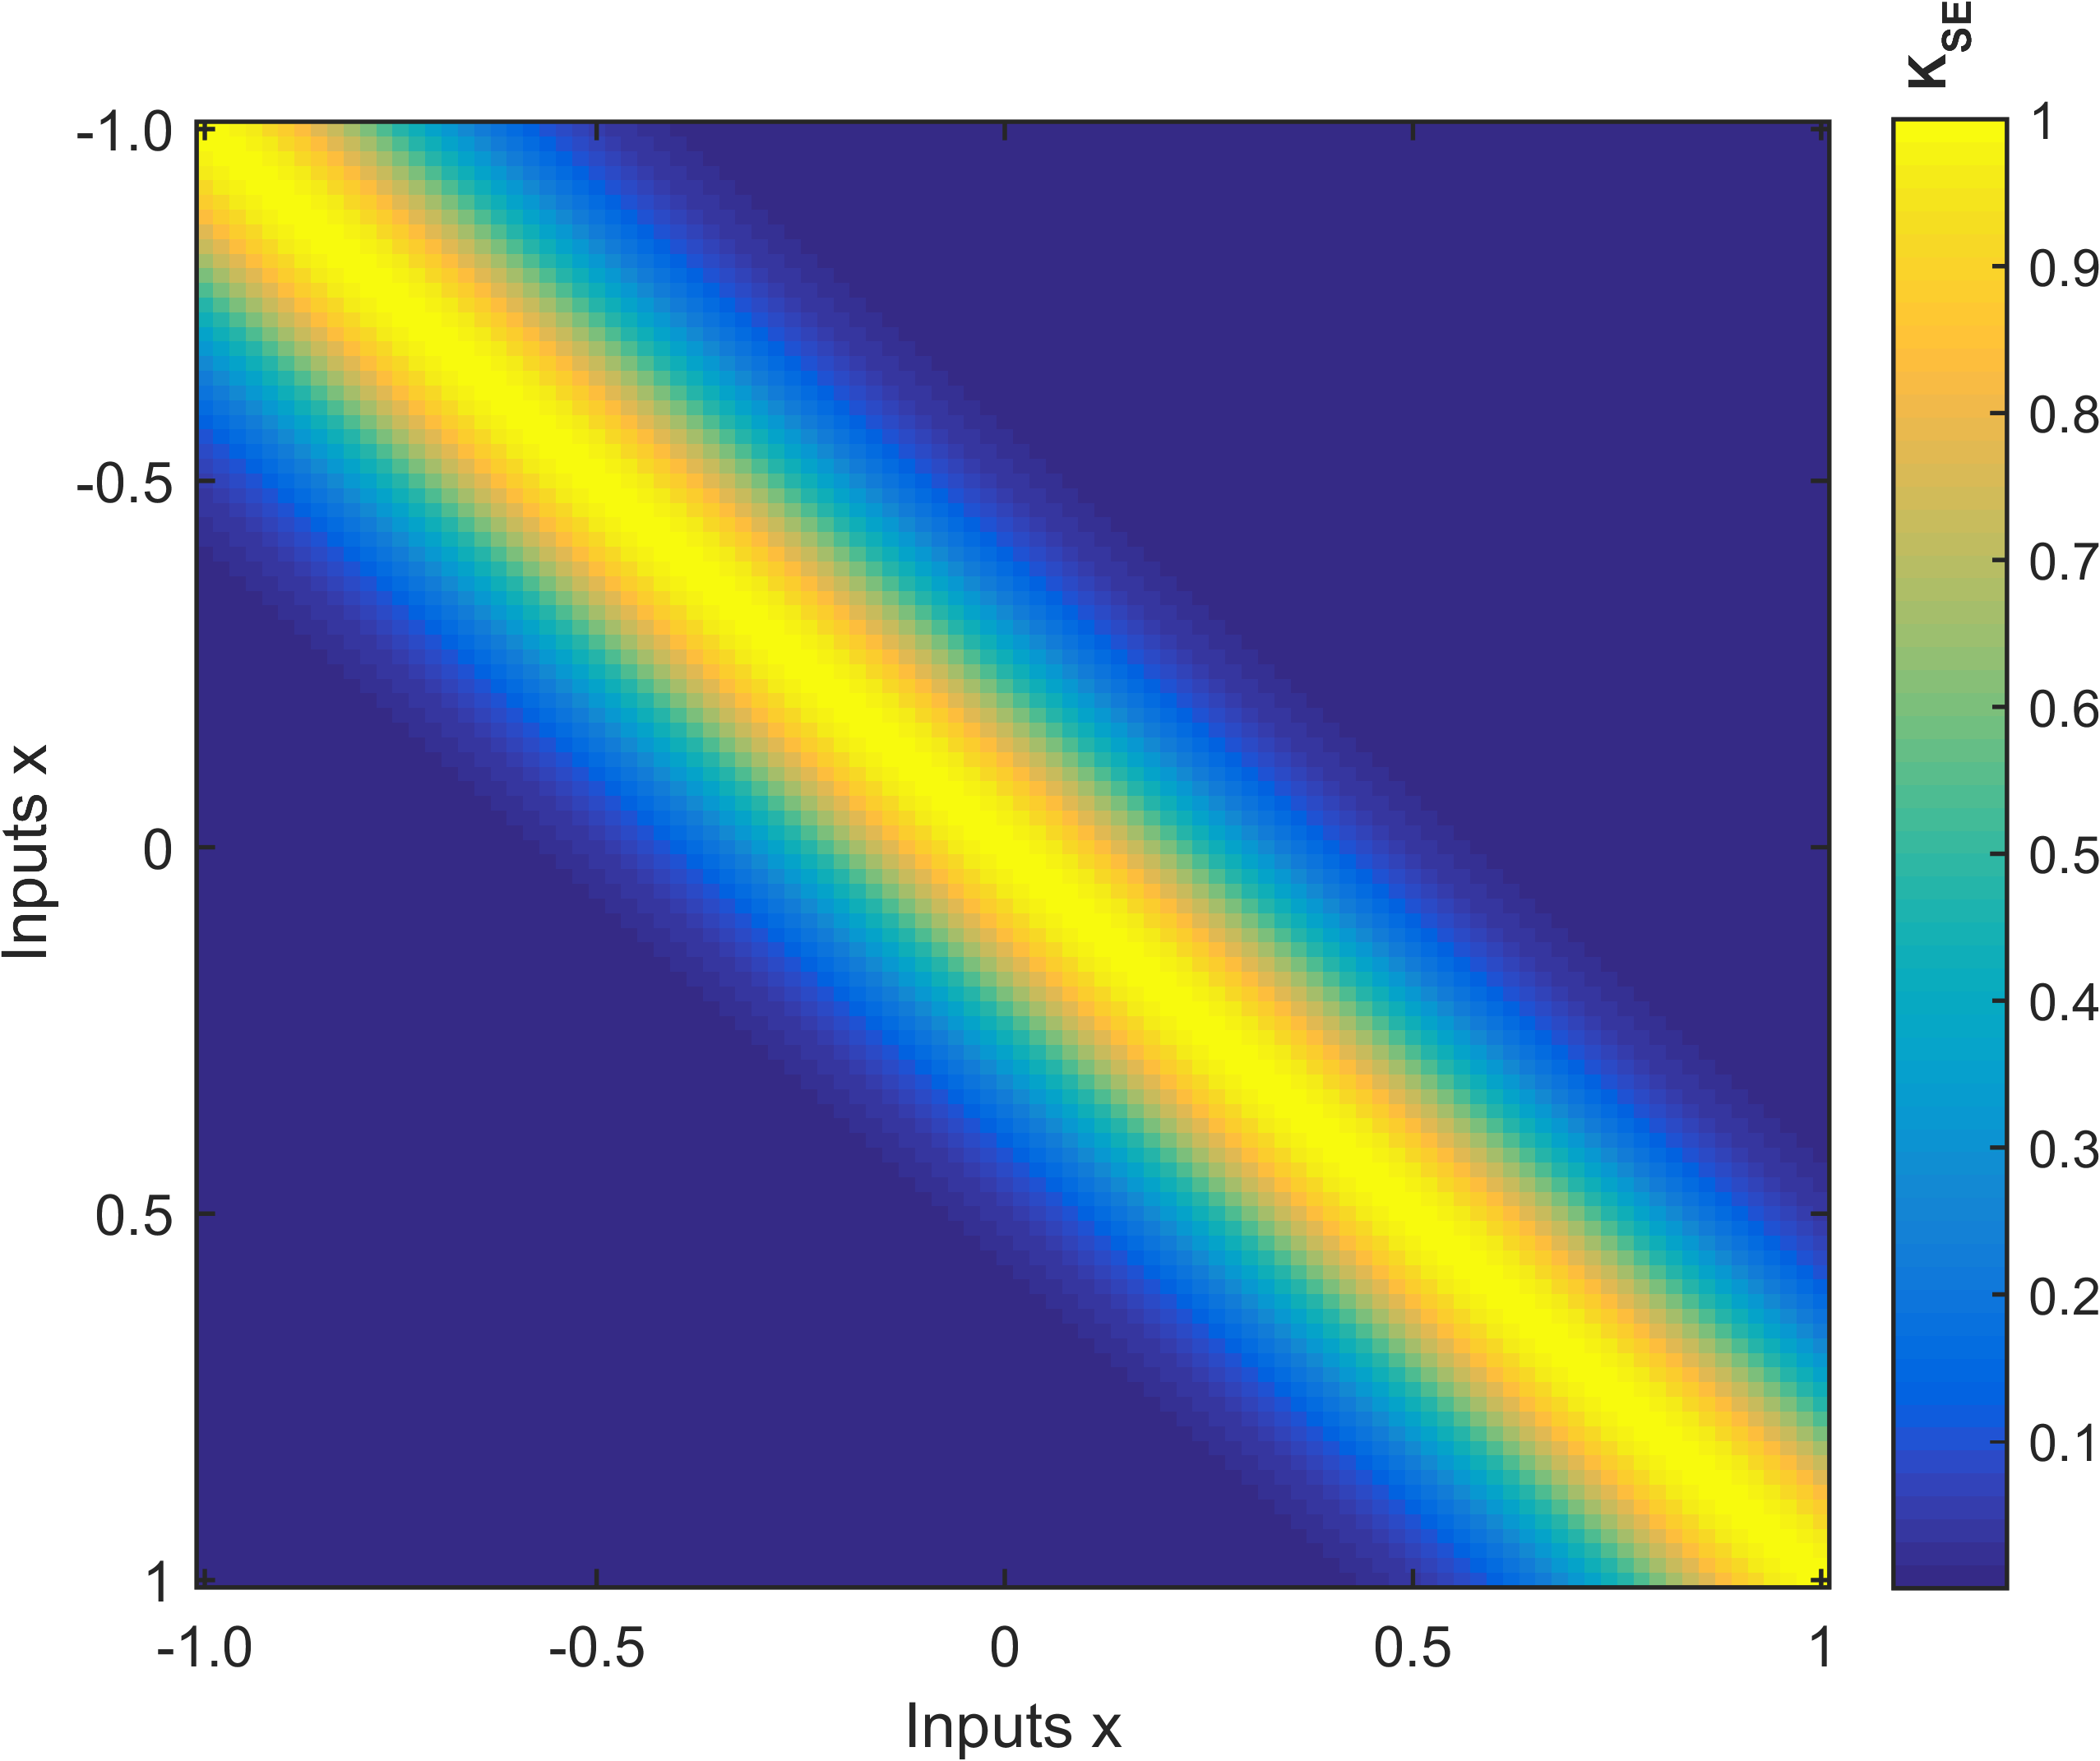
\includegraphics[width=0.45\textwidth]
        {images/part1/covSEmatrix_1}
        \label{subFigcovSEmatrix_1}
  }\quad
\subfigure[{Covariance matrix for a SE kernel with $(\VEC{\theta} = [1, 0.5])$ at the input points $\myMatrix{X^{*}} = \{[0:0.02:1]\}$}]
  {
        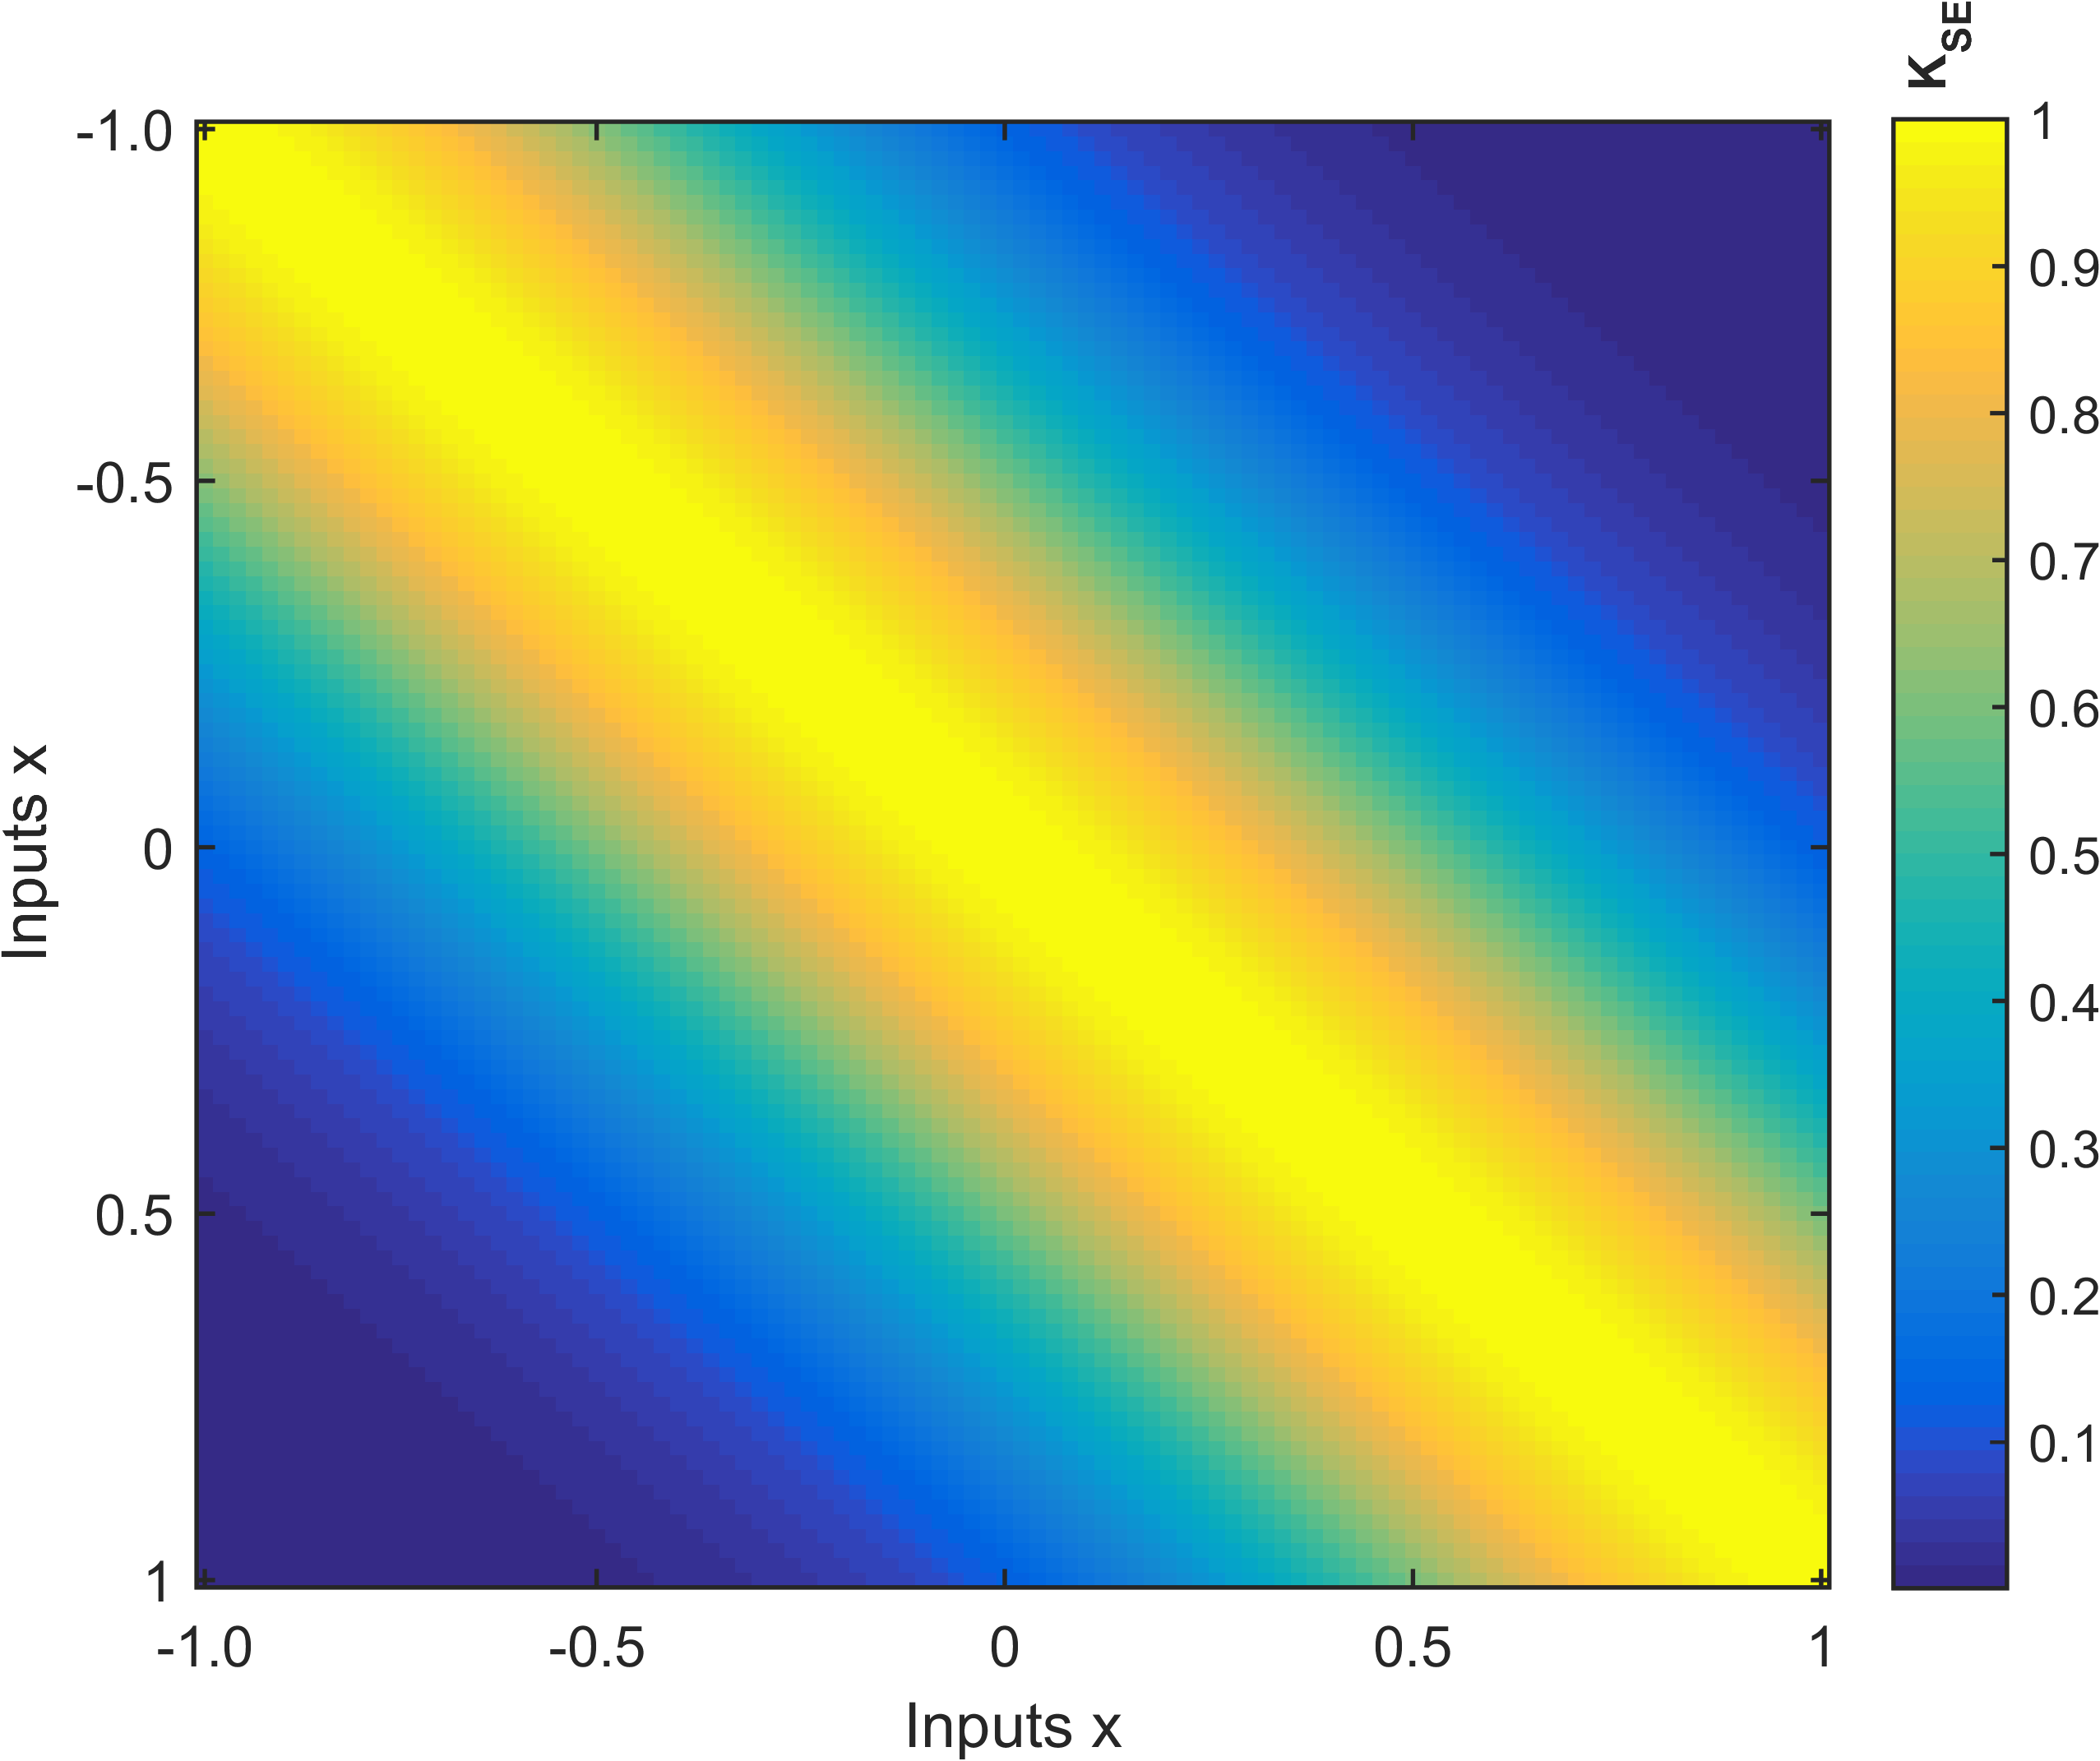
\includegraphics[width=0.45\textwidth]
        {images/part1/covSEmatrix_2}
        \label{subFigcovSEmatrix_2}
  }\quad
  
       \caption{Covariance matrix for a SE kernel with different hyper-parameters at the input points $\myMatrix{X^{*}} = \{[0:0.02:1]\}$. The SE kernel of figure \ref{subFigcovSEmatrix_1} has a lower length-scale than figure \ref{subFigcovSEmatrix_2}. Notice how the covariance values are more spread out for figure \ref{subFigcovSEmatrix_2}.}\label{figGPCovarianceMatrix}
\end{figure}

\marginnote{\textsl{Random Draw}}[1cm]
To generate a random Gaussian vector $\VEC{f(X_{*})}$ of length $N_{*}$, we first calculate the Cholesky decomposition\footnote{Cholesky Decomposition is also called the square-root of matrix and is defined for positive definite matrices} of the covariance matrix $\myMatrix{K(X_{*}, X_{*})} = \myMatrix{L}\myMatrix{L^{T}}$, where $\myMatrix{L}$ is a lower triangular matrix. We then generate a random vector $\VEC{u}$, such that $\VEC{u} = \mathcal{N}(0, \myMatrix{I_{N_*}})$ and $\myMatrix{I_{N_*}}$ is an identity matrix of size $N_{*} \times N_{*}$.  The random vector can then be computed as $\VEC{f(X_{*})} = \VEC{m(X_{*})} + \myMatrix{L}\VEC{u}$, and when plotted with the inputs $\myMatrix{X_{*}}$, gives a randomly drawn function. The Matlab Code \ref{codeSamplingFUnction} shows how can we draw functions randomly from a GP prior.
% Adding the algorithm

\begin{mdframed}[hidealllines=true,backgroundcolor=lightgray!20]
\lstinputlisting[caption={Sampling a random function from the prior}, 
                    captionpos=b, 
                    label={codeSamplingFUnction}, 
                    backgroundcolor = \color{MatlabCellColour}, 
                    style=Matlab-editor,
                    basicstyle=\color{black}\ttfamily\small]
                    {codes/chapter2/samplingFunctionFromAPrior.m}
\end{mdframed}

\marginnote{\textsl{Figure \ref{figGPPriors}}}[1cm]
Figure \ref{figGPPriors} shows 5 random functions drawn for a zero mean GP with the covariance matrices of figure \ref{figGPCovarianceMatrix}. The solid black line defines the mean function, shaded blue region defines 95\% confidence interval (2$\sigma$) distance away from the mean. The dashed lines represent five functions drawn at random from a GP prior. We can observe that figure \ref{subFigSEPrior_1} varies faster when compared to figure \ref{subFigSEPrior_2} due to smaller length scale hyper-parameter. 

\begin{figure}[!ht]
  \centering
    \subfigure[{Draws from a GP prior with mean zero and SE Kernel with $(\VEC{\theta} = [1, 0.2])$. }]
  {
        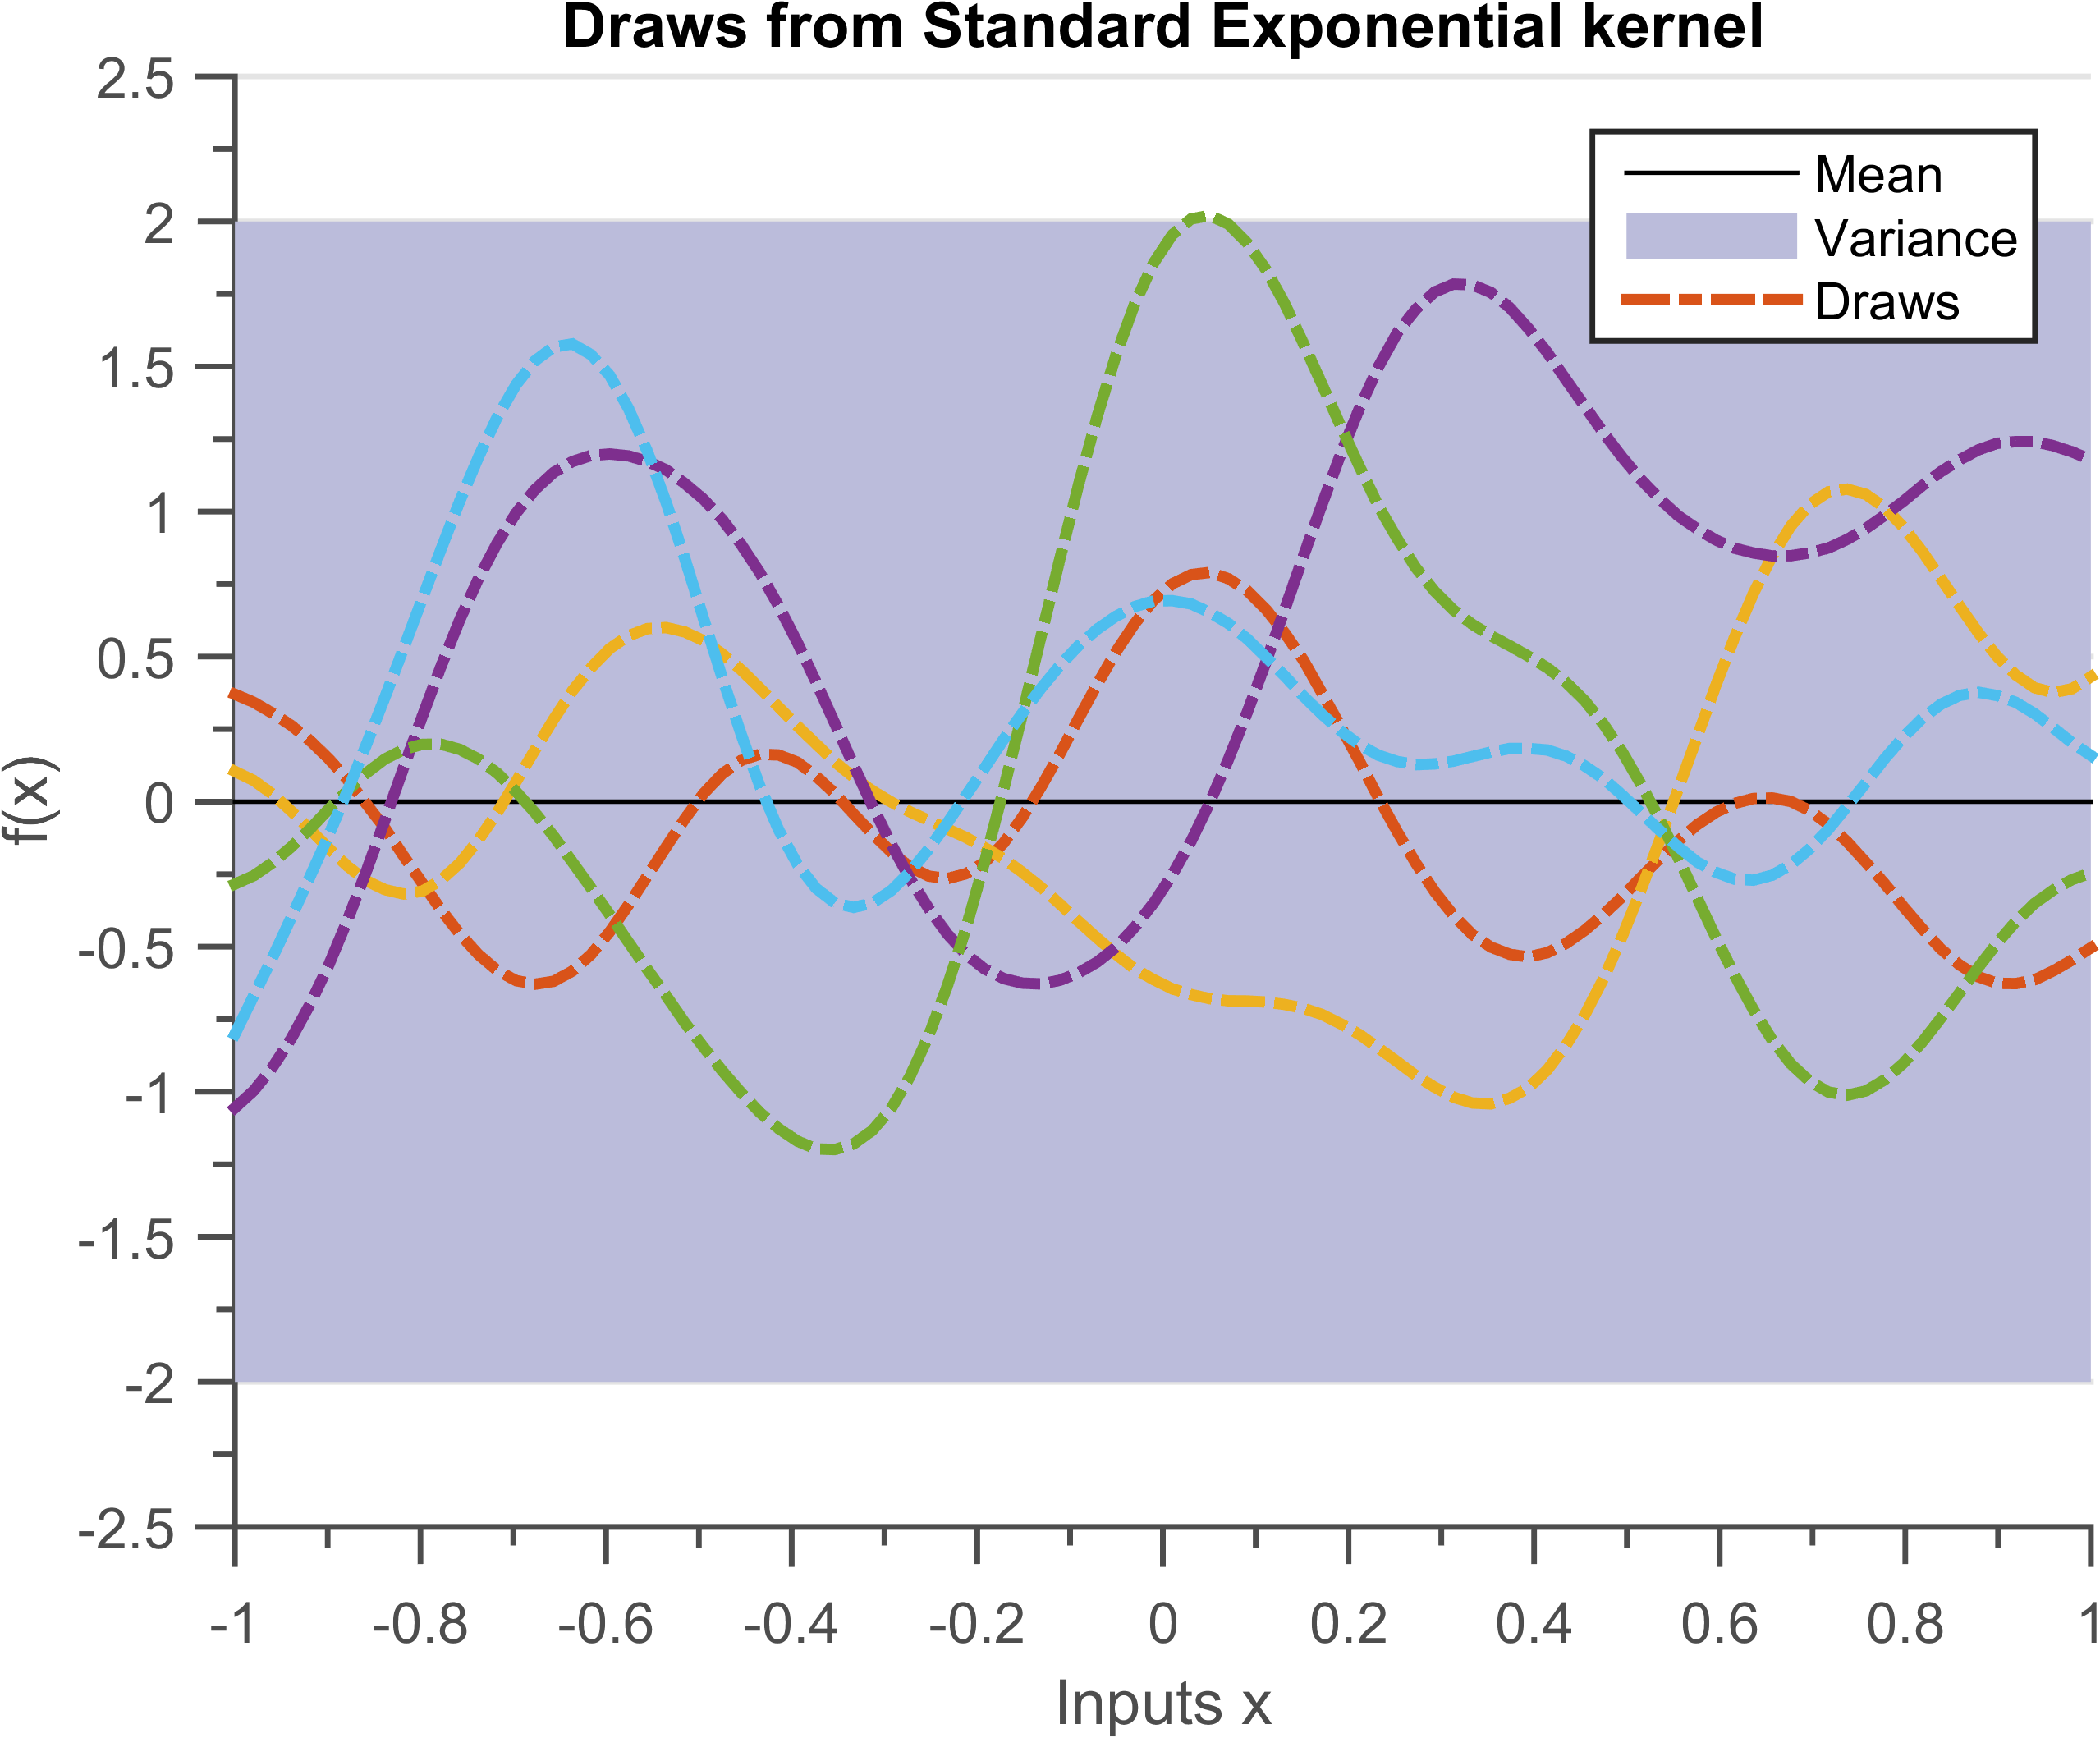
\includegraphics[width=0.45\textwidth]
        {images/part1/drawsSEKernel_1}
        \label{subFigSEPrior_1}
  }\quad
\subfigure[{Draws from a GP prior with mean zero and SE kernel with $(\VEC{\theta} = [1, 0.5])$}]
  {
        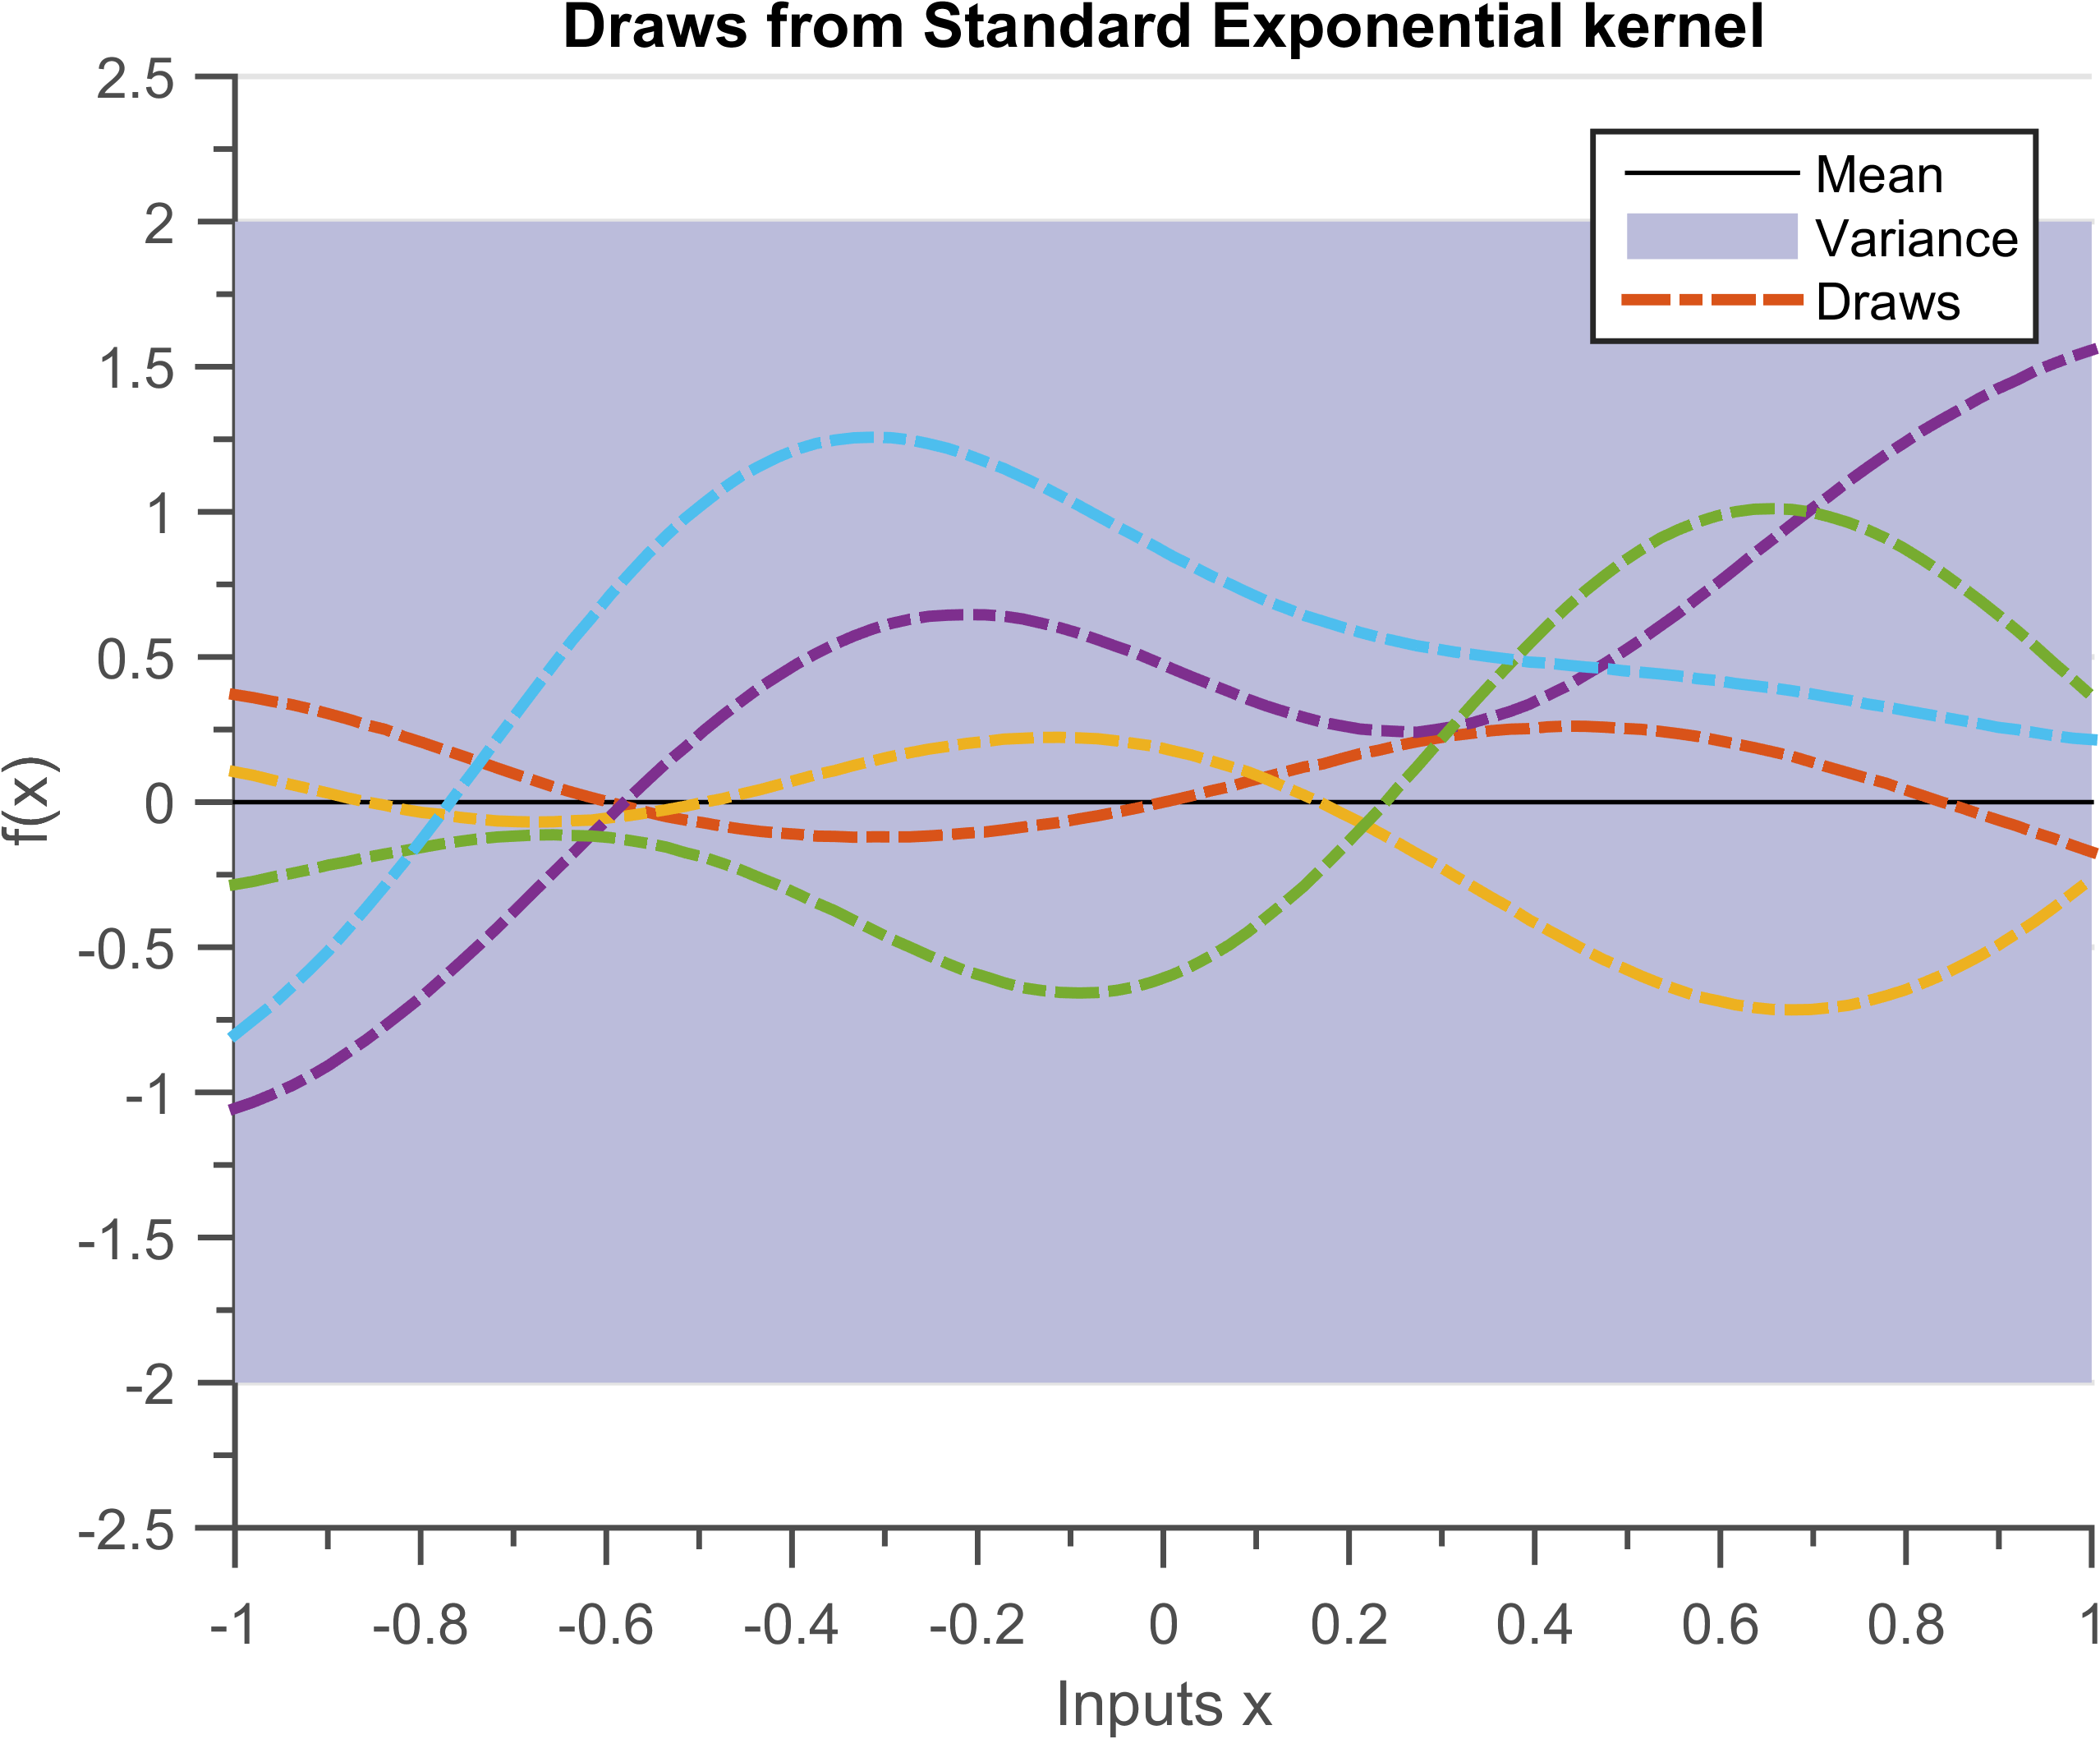
\includegraphics[width=0.45\textwidth]
        {images/part1/drawsSEKernel_2}
        \label{subFigSEPrior_2}
  }\quad
  
       \caption{The solid black line defines the mean function, shaded blue region defines 95\% confidence interval (2$\sigma$) distance away from the mean. The dashed lines represent five functions drawn at random from a GP prior. We can observe that figure \ref{subFigSEPrior_1} varies faster when compared to figure \ref{subFigSEPrior_2} due to smaller length scale hyper-parameter.       }\label{figGPPriors}
\end{figure}



\section{Posterior}\label{secPosterior}
Once we have defined an appropriate prior we wish to incorporate the information of the training data set into the probabilistic framework. In the Bayesian framework, a posterior is the probability distribution after updating the information of evidence into prior distribution. 


\subsection{Posterior with Noise-free observations}\label{subSecPosteriorNoiseFree}
We first consider the case of noise-free observations, that is $y(x_{i}) = f_{i}$ $ \forall i \in [1; N] \}$. This is the case while interpolating computer simulations since their outputs can be treated as having no noise \cite{sacks1989design}. If we desire to interpolate at test points $\myMatrix{X_{*}}$, then the joint distribution of the training outputs $\VEC{f(X)}$ and test outputs $\VEC{f(X_{*})}$ is given by equation \ref{equationJointPriorNoiseFree}.

\begin{equation}\label{equationJointPriorNoiseFree}
\Pr\left [ \begin{matrix}
\VEC{f(X)}
\\ \VEC{f(X_{*})}
\end{matrix} \right ] = 
\mathcal{N}\left (\left [ \begin{matrix} 0 \\ 0 \end{matrix} \right ]
, 
\left [ \begin{matrix}
\myMatrix{K(X, X)} & \myMatrix{K(X, X_{*})}\\ 
\myMatrix{K(X_{*}, X)} & \myMatrix{K(X_{*}, X_{*})}
\end{matrix} \right ]
\right)
\end{equation}

$\myMatrix{K(X, X_{*})}$ is $N \times N_{*}$ covariance matrix between the training points $\myMatrix{X}$ and test points $\myMatrix{X_{*}}$ (equation \ref{eqnCovMatrixSquaredExponential}). The other covariance matrices $\myMatrix{K(X, X)}$, $\myMatrix{K(X_{*}, X)}$ and $\myMatrix{K(X_{*}, X_{*})}$ can be computed similarly. 

\marginnote{\textsl{Conditioned distribution}}[1cm]
The posterior will be the conditional probability of $\VEC{f(X_{*})}$ given the prior and data set. For a multi-variate Gaussian prior the conditional posterior distribution is also a multi-variate Gaussian and can be calculated tractably. For a more detailed derivation refer to appendix \textbf{refer to the appendix here}. Graphically, we can imagine that the Bayes theorem is removing all the functions from our prior family of functions that do not pass through the data set (figure \ref{figGPNoiseLessPosteriors}). The predicted distribution after adding the information of data set into the prior can be written as:

  \begin{equation}\label{eqNoiseFreePosteriorGP}
  \begin{aligned}
  \Pr(\VEC{f(X_{*}}) \mid \myMatrix{X_{*}}, \myMatrix{X}, \VEC{f(X)}) = GP(  & \myMatrix{K(X_{*}, X)}( \myMatrix{K(X, X)} )^{-1}\VEC{f(X)},   \\ 
                                & \myMatrix{K(X_{*}, X_{*})} - \myMatrix{K(X_{*}, X)}( \myMatrix{K(X, X)} )^{-1} \myMatrix{K(X, X_{*})})
  \end{aligned}
  \end{equation}

The term $\myMatrix{K(X_{*}, X)}( \myMatrix{K(X, X)} )^{-1}\VEC{f(X)}$ is the predicted mean of the posterior at the test points $\myMatrix{X_{*}}$. The term $ \myMatrix{K(X_{*}, X_{*})} - \myMatrix{K(X_{*}, X)}( \myMatrix{K(X, X)} )^{-1} \myMatrix{K(X, X_{*})}$ is the predicted covariance. 

We again use the dataset $\mathcal{D}_{1}$ (earlier used in section \ref{secBayesianModelling}) to calculate the posterior distribution. The Matlab Code \ref{codePosterior} shows how to calculate the posterior mean and variance. Notice that calculating the posterior mean and variance are only a few lines of code. 

.% Adding the algorithm
\begin{mdframed}[hidealllines=true,backgroundcolor=lightgray!20]
\lstinputlisting[caption={Calculating and plotting the mean, the variance and a sample of the posterior}, 
                    captionpos=b, 
                    label={codePosterior}, 
                    backgroundcolor = \color{MatlabCellColour},
                    style=Matlab-editor,
                    basicstyle=\color{black}\ttfamily\small]
                    {codes/chapter2/evaluatingAndPlottingThePosterior.m}
\end{mdframed}

Figure \ref{figGPNoiseLessPosteriors} shows the posterior GP after adding observed data into the initial prior. We can see that thanks to the Bayes theorem all the functions that do not pass through the data, are eliminated from the hypothesis space. The solid black line defines the mean function, blue region defines 95\% confidence interval (2$\sigma$) distance away from the mean. The mean of the posterior distribution is also used as a point estimate for interpolation. The dashed lines represent three functions drawn at random from a GP posterior. Random functions can be sampled from the posterior distribution as described in the earlier section. 


\begin{figure}[!ht]
  \centering
    \subfigure[{Posterior distribution for the case of noiseless observations. Prior is a GP with mean zero and covariance as SE Kernel with $(\VEC{\theta} = [1, 0.2])$, data set is $\{x = -0.5; f = 0\}$.}]
  {
        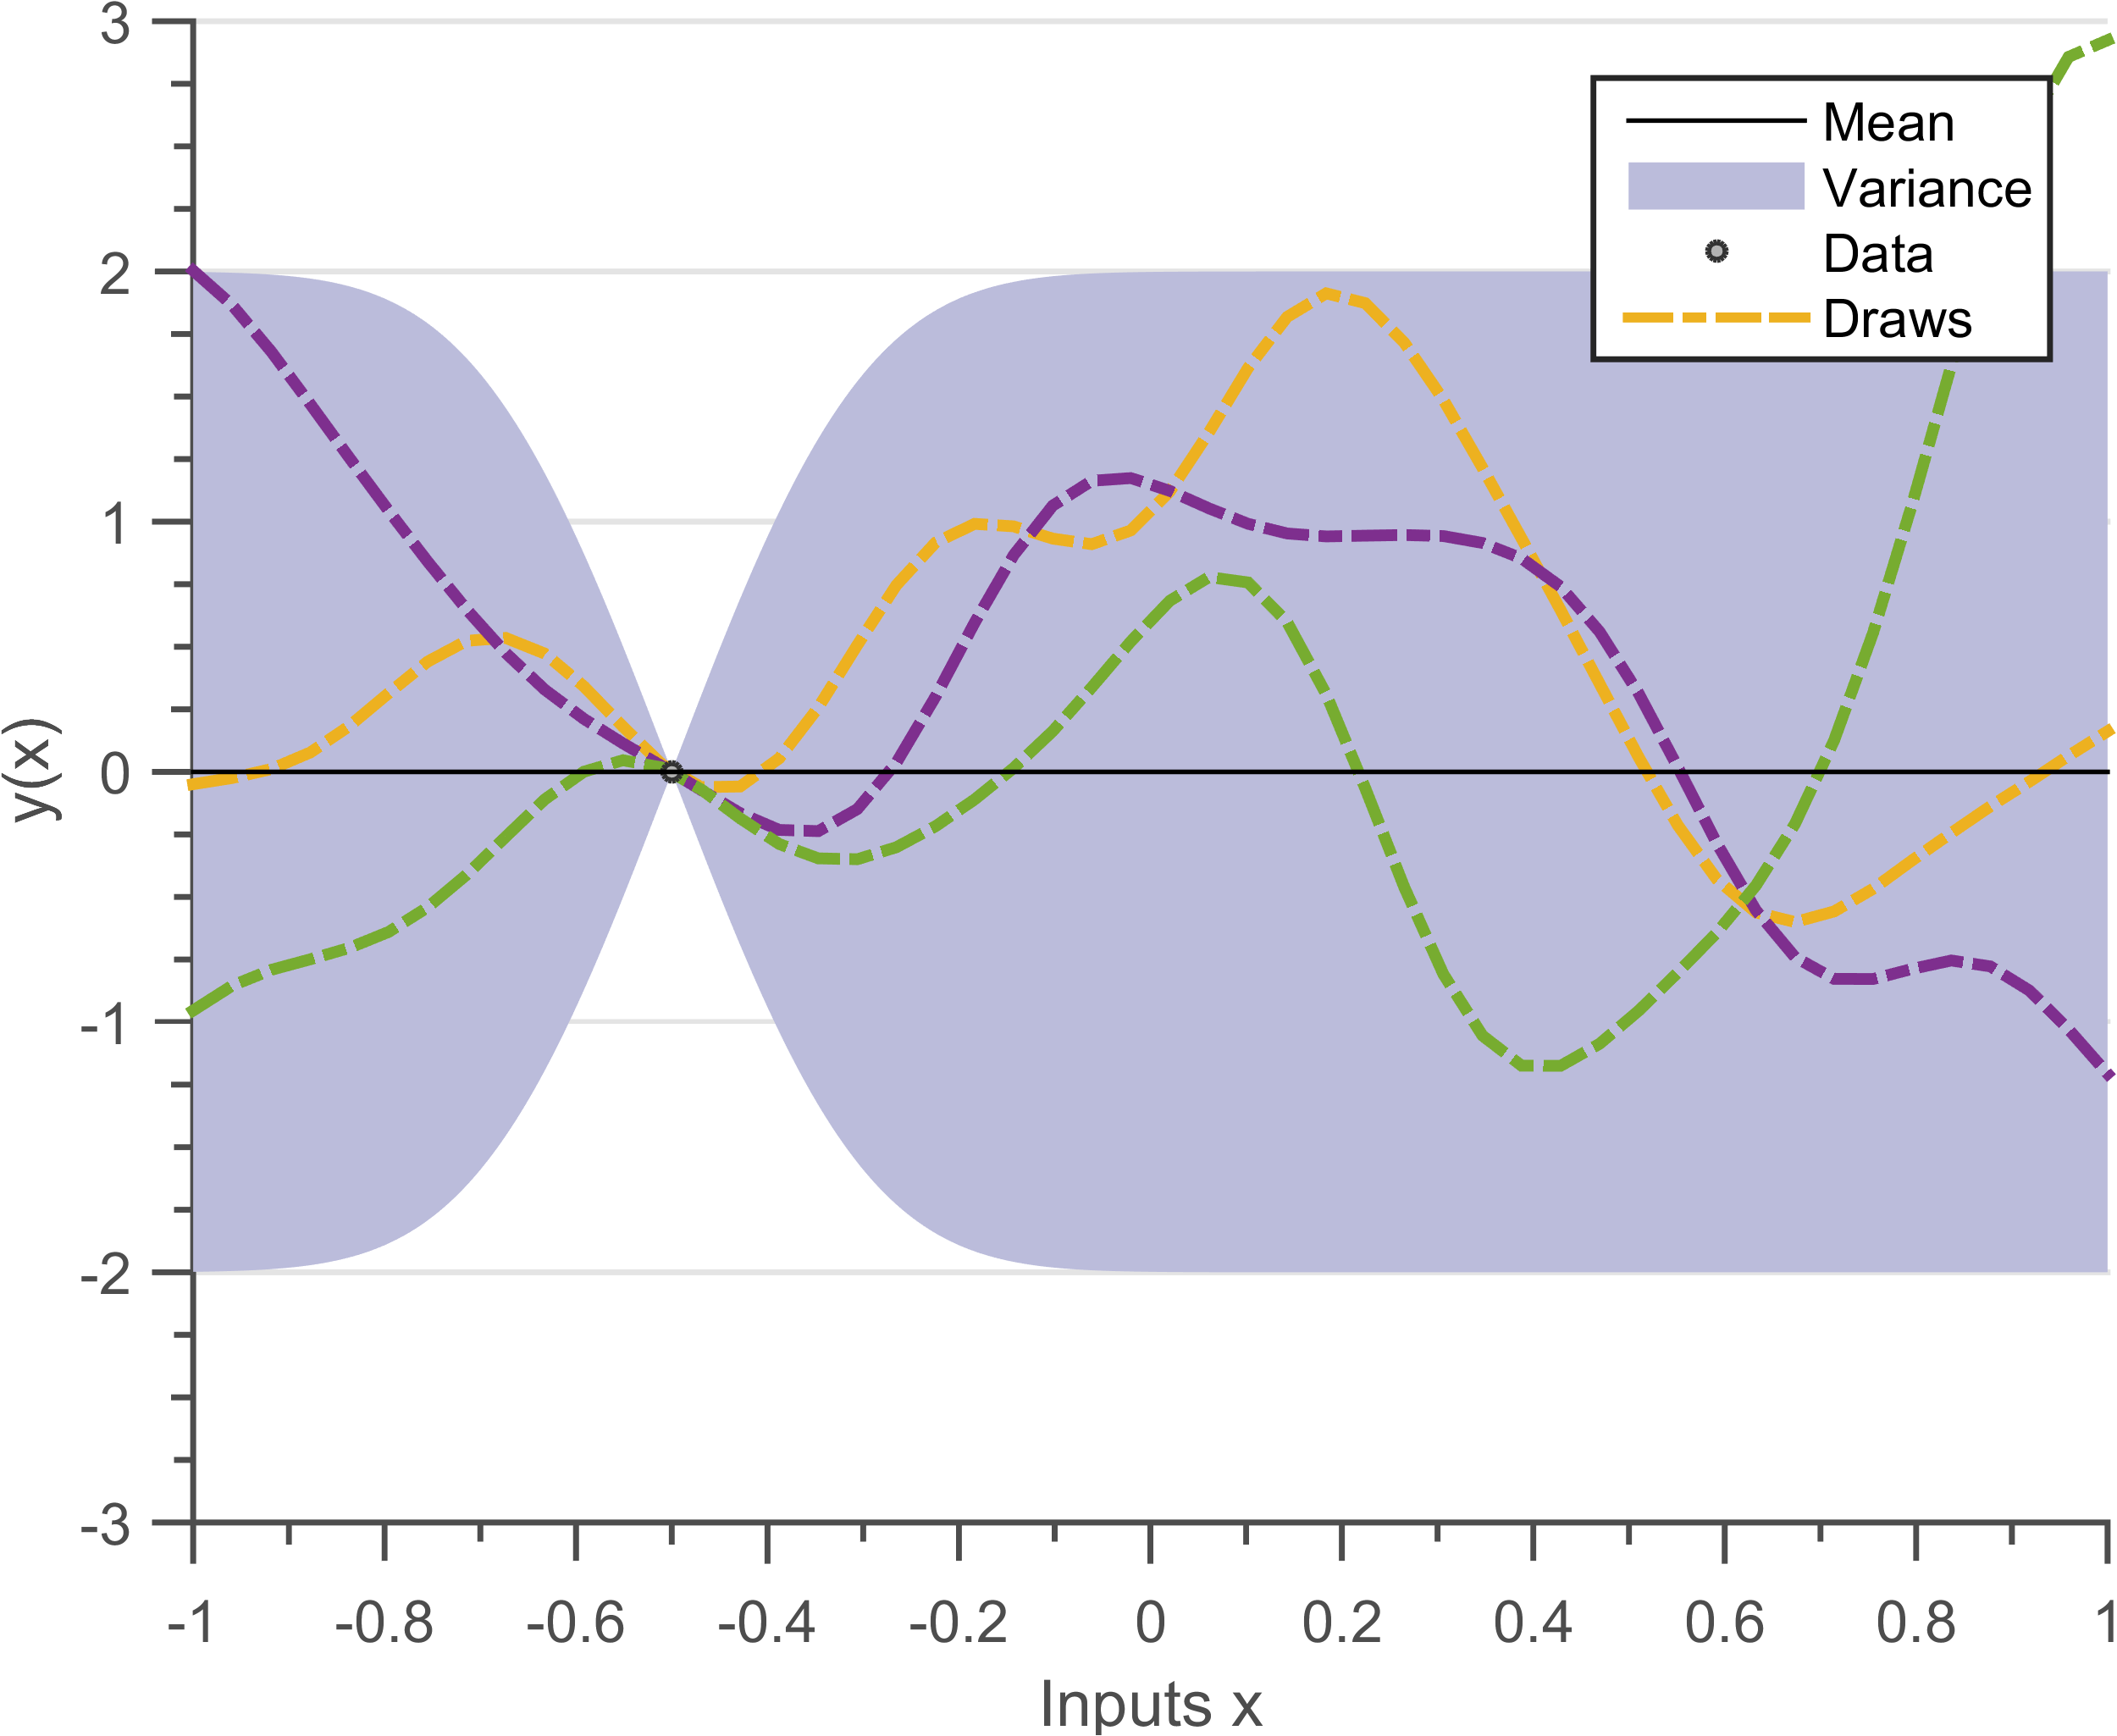
\includegraphics[width=0.45\textwidth]
        {images/part1/posteriorSENoiseLess_1}
        \label{posteriorSENoiseLess_1}
  }\quad
\subfigure[{Posterior distribution for the case of noiseless observations. Prior is a GP with mean zero and covariance as SE Kernel with $(\VEC{\theta} = [1, 0.2])$, data set is $\{x = [-0.5, 0.33, 0.66]; f = [0, 0.5, 0.5]\}$}.  ]
  {
        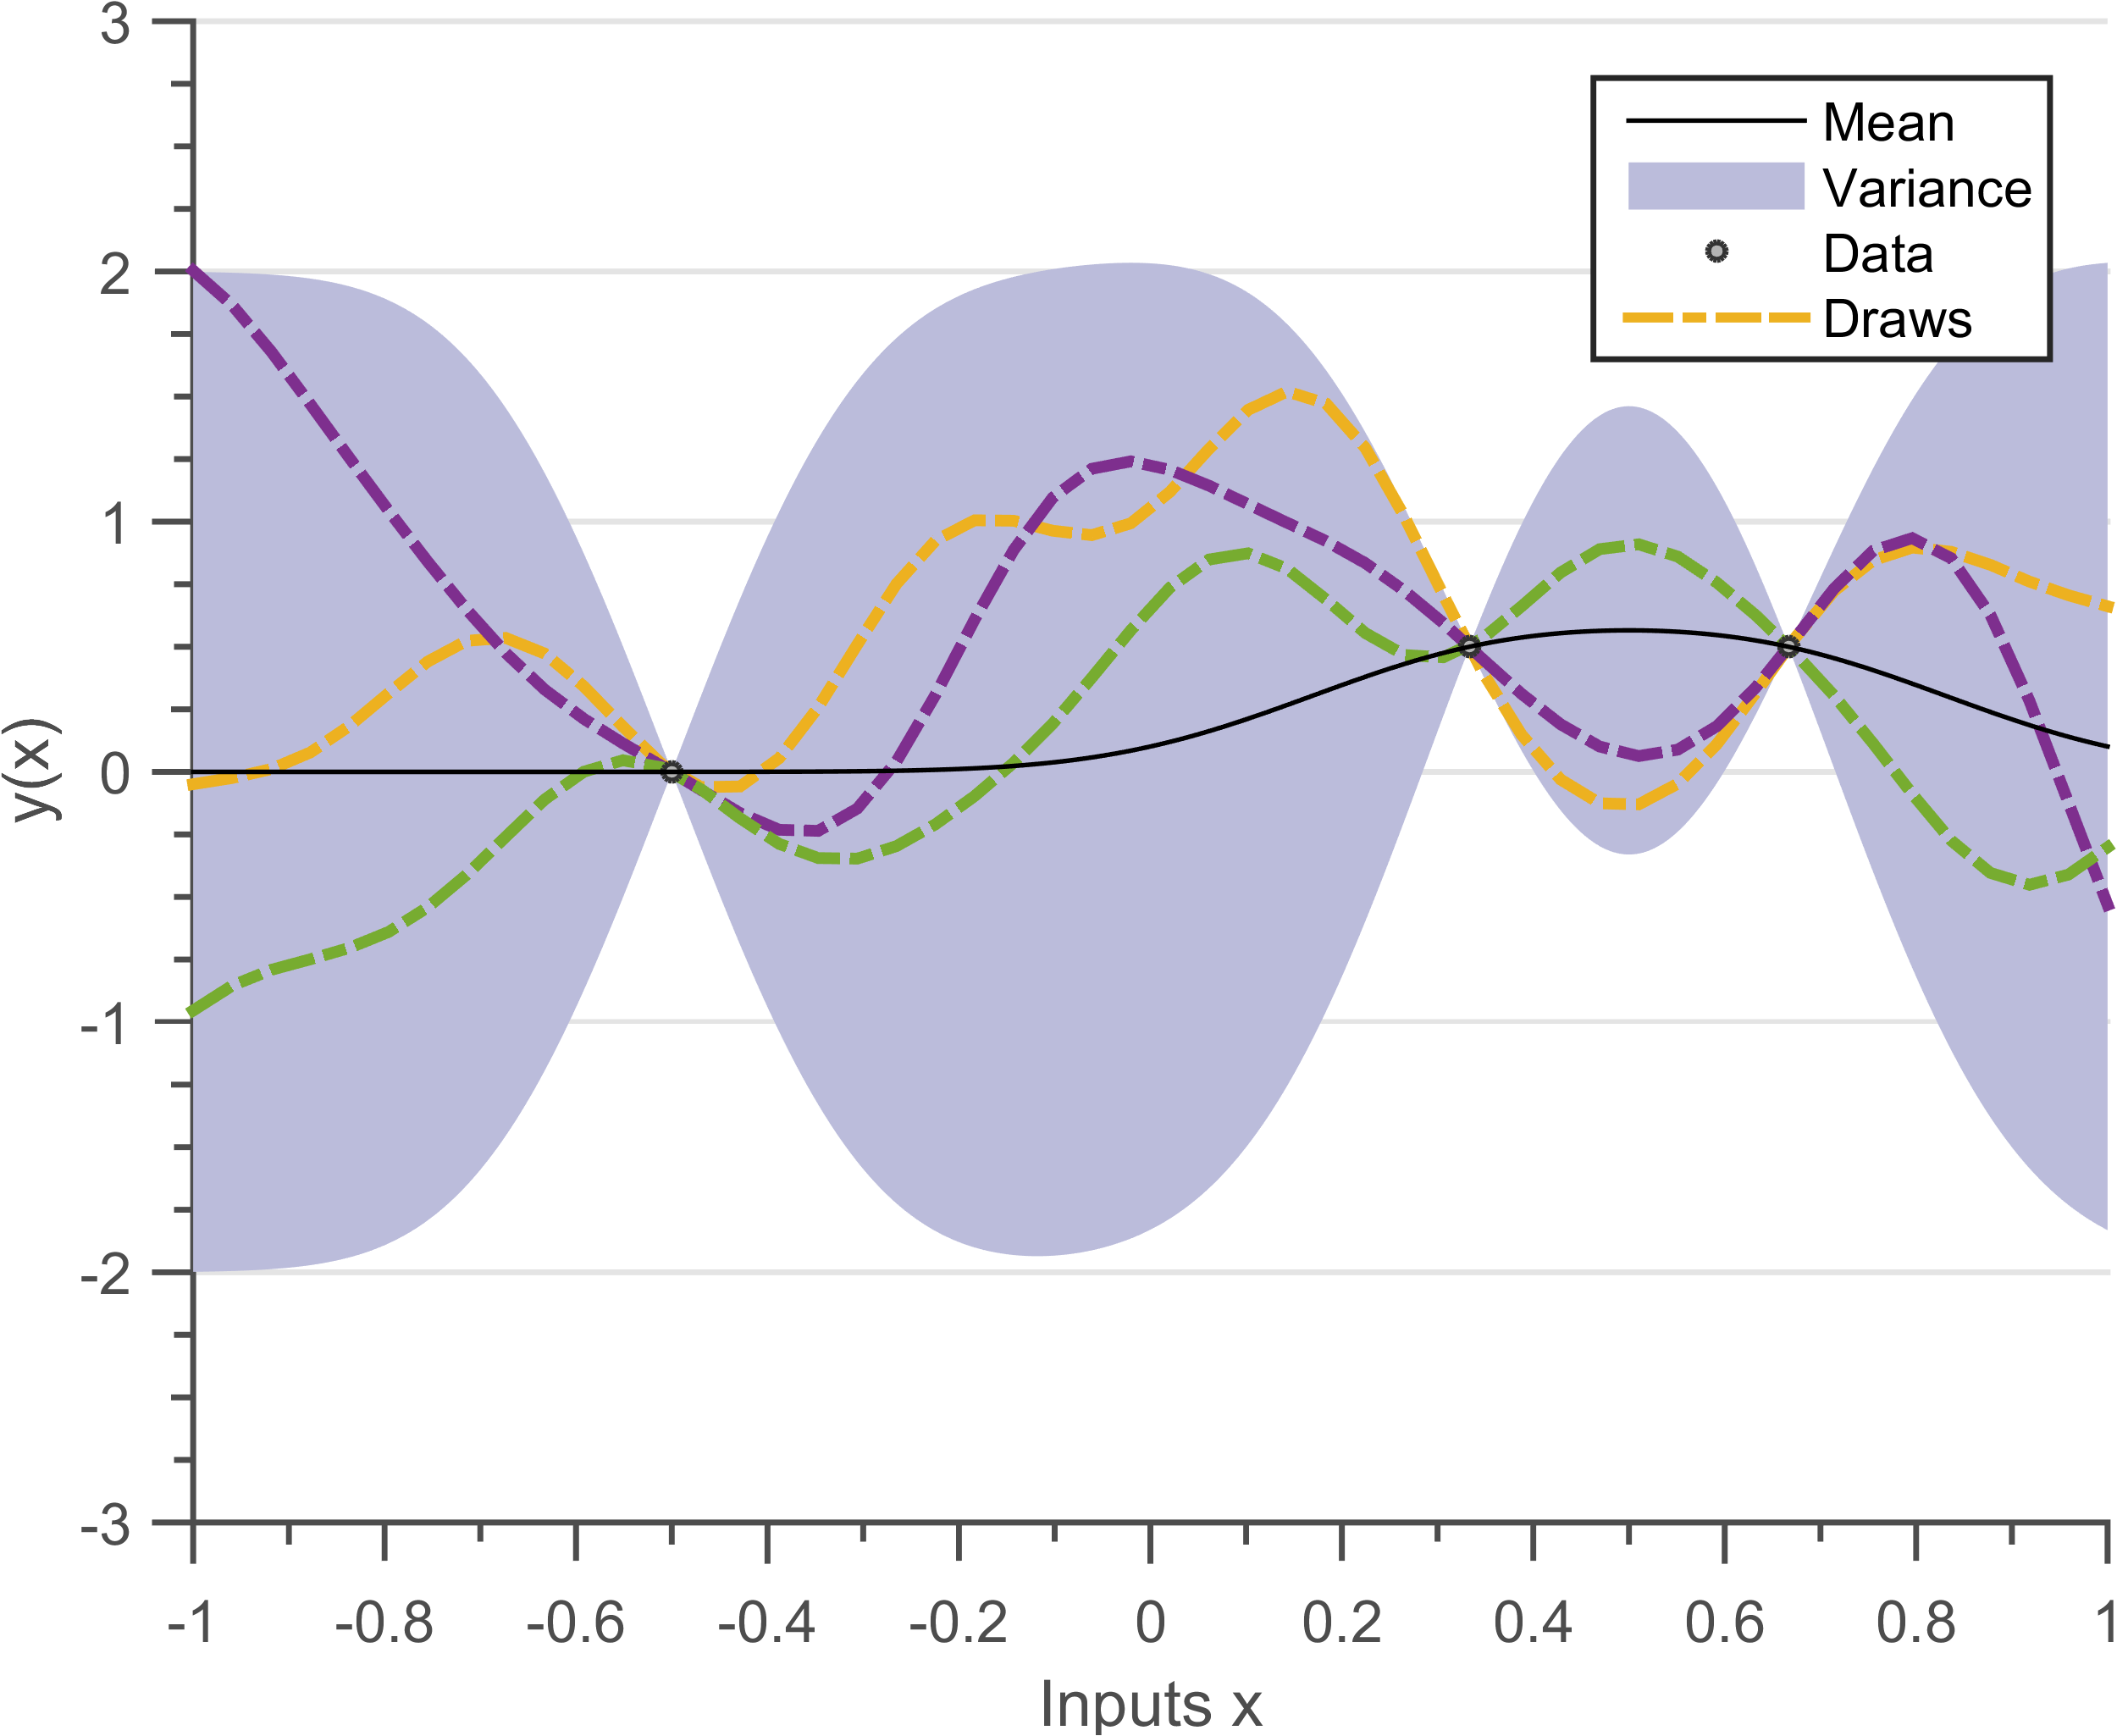
\includegraphics[width=0.45\textwidth]
        {images/part1/posteriorSENoiseLess_3}
        \label{posteriorSENoiseLess_3}
  }\quad
  
       \caption{Prediction in the case of noiseless observations. The solid black line defines the mean function, blue region defines 95\% confidence interval (2$\sigma$) distance away from the mean. The dashed lines represent three functions drawn at random from a GP posterior. We can observe that Bayes Theorem eliminates all the functions that do not pass through the observed data-set.}
       \label{figGPNoiseLessPosteriors}
\end{figure}



\subsection{Posterior with Noisy observations}\label{subSecPosteriorNoisy}
If we assume a more general case of noisy observations, then the measured outputs can be written as:

\begin{equation}\label{eqNoiseEquation}
y(\VEC{x}) = f(\VEC{x}) + \epsilon
\end{equation}

Such that $\epsilon$ is an independent random noise sampled from a white noise Gaussian $\mathcal{N}(0, \sigma_{n}^{2})$. We can thus write the prior GP of the noisy case as:

\begin{equation}\label{equationMeanZeroGPNoisydefinition}
\Pr[y(\VEC{x})] = GP(0 , k(\VEC{x_1}, \VEC{x_2}) + \sigma^{2}_{n}\delta_{x_{1}x_{2}})
\end{equation}

Here, $\delta_{x_{1}x_{2}}$ is a Kronecker delta function, which is one if $x_1 = x_2$ and zero otherwise. Since the noise is independent for each observation, there is no noise term for covariances across inputs. The joint distribution of the training outputs $\VEC{y(X)}$ and true physical process $\VEC{f(X_{*})}$ according to the above prior becomes:

\begin{mdframed}[hidealllines=true,backgroundcolor=lightgray!20]
\lstinputlisting[caption={Matlab code for a noisy SE covariance function}, 
                    captionpos=b, 
                    label={codeNoisySE}, 
                    backgroundcolor = \color{MatlabCellColour},
                    style=Matlab-editor,
                    basicstyle=\color{black}\ttfamily\small]
                    {codes/chapter2/noisySEKernel.m}
\end{mdframed}

\begin{equation}\label{equationJointPriorNoisy}
\Pr\left [ \begin{matrix}
\VEC{y(X)}
\\ \VEC{f(X_{*})}
\end{matrix} \right ]
= 
\mathcal{N}\left (
\left [ \begin{matrix}
0
\\ 0

\end{matrix} \right ] , \left [ \begin{matrix}
\myMatrix{K(X, X)} + \sigma^{2}_{n}\myMatrix{I_N} & \myMatrix{K(X, X_{*})}\\ 
\myMatrix{K(X_{*}, X)} & \myMatrix{K(X_{*}, X_{*})}
\end{matrix} \right ] 
\right )
\end{equation}

The difference between equation \ref{equationJointPriorNoisy} and \ref{equationJointPriorNoiseFree} is the addition of noise term $\sigma^{2}_{n}\myMatrix{I_N}$. Since the noise at each measurement point is assumed to be independent, it is multiplied to an identity matrix. To know how to add more complex noise models please refer to section \ref{chapCombiningBasicCovariances}. The posterior distribution of $f(X_{*})$ can be calculated as:

  \begin{equation}\label{eqNoisyPredictiveGP}
  \begin{aligned}
  \Pr(\VEC{f(X_{*}}) \mid \myMatrix{X_{*}}, \myMatrix{X}, \VEC{y(X)}) = GP(  & \myMatrix{K(X_{*}, X)}( \myMatrix{K(X, X)} + \sigma^{2}_{n}\myMatrix{I_N} )^{-1}\VEC{f(X)},   \\ 
                                & \myMatrix{K(X_{*}, X_{*})} - \myMatrix{K(X_{*}, X)}( \myMatrix{K(X, X)} + \sigma^{2}_{n}\myMatrix{I_N} )^{-1} \myMatrix{K(X, X_{*})})
  \end{aligned}
  \end{equation}


Figure \ref{figGPNoisyPosteriors} shows the posterior GP after adding observed data into the initial prior. The solid black line defines the mean function, blue region defines 95\% confidence interval (2$\sigma$) distance away from the mean. The dashed lines represent three functions drawn at random from a GP posterior. Random functions can be sampled from the posterior distribution as described in the earlier section \ref{secPrior}.  Due to the inclusion of noise in the prior, we see that the draws from posterior are not necessarily passing through the observed point.

\begin{figure}[!ht]
  \centering
    \subfigure[{Posterior distribution for the case of noisy observations. Prior is a GP with mean zero, covariance as SE Kernel with $(\VEC{\theta} = [1, 0.2])$ and noise as $\sigma_{n} = [0.02])$, , data set is $\{x = -0.5; f = 0\}$.}]
  {
        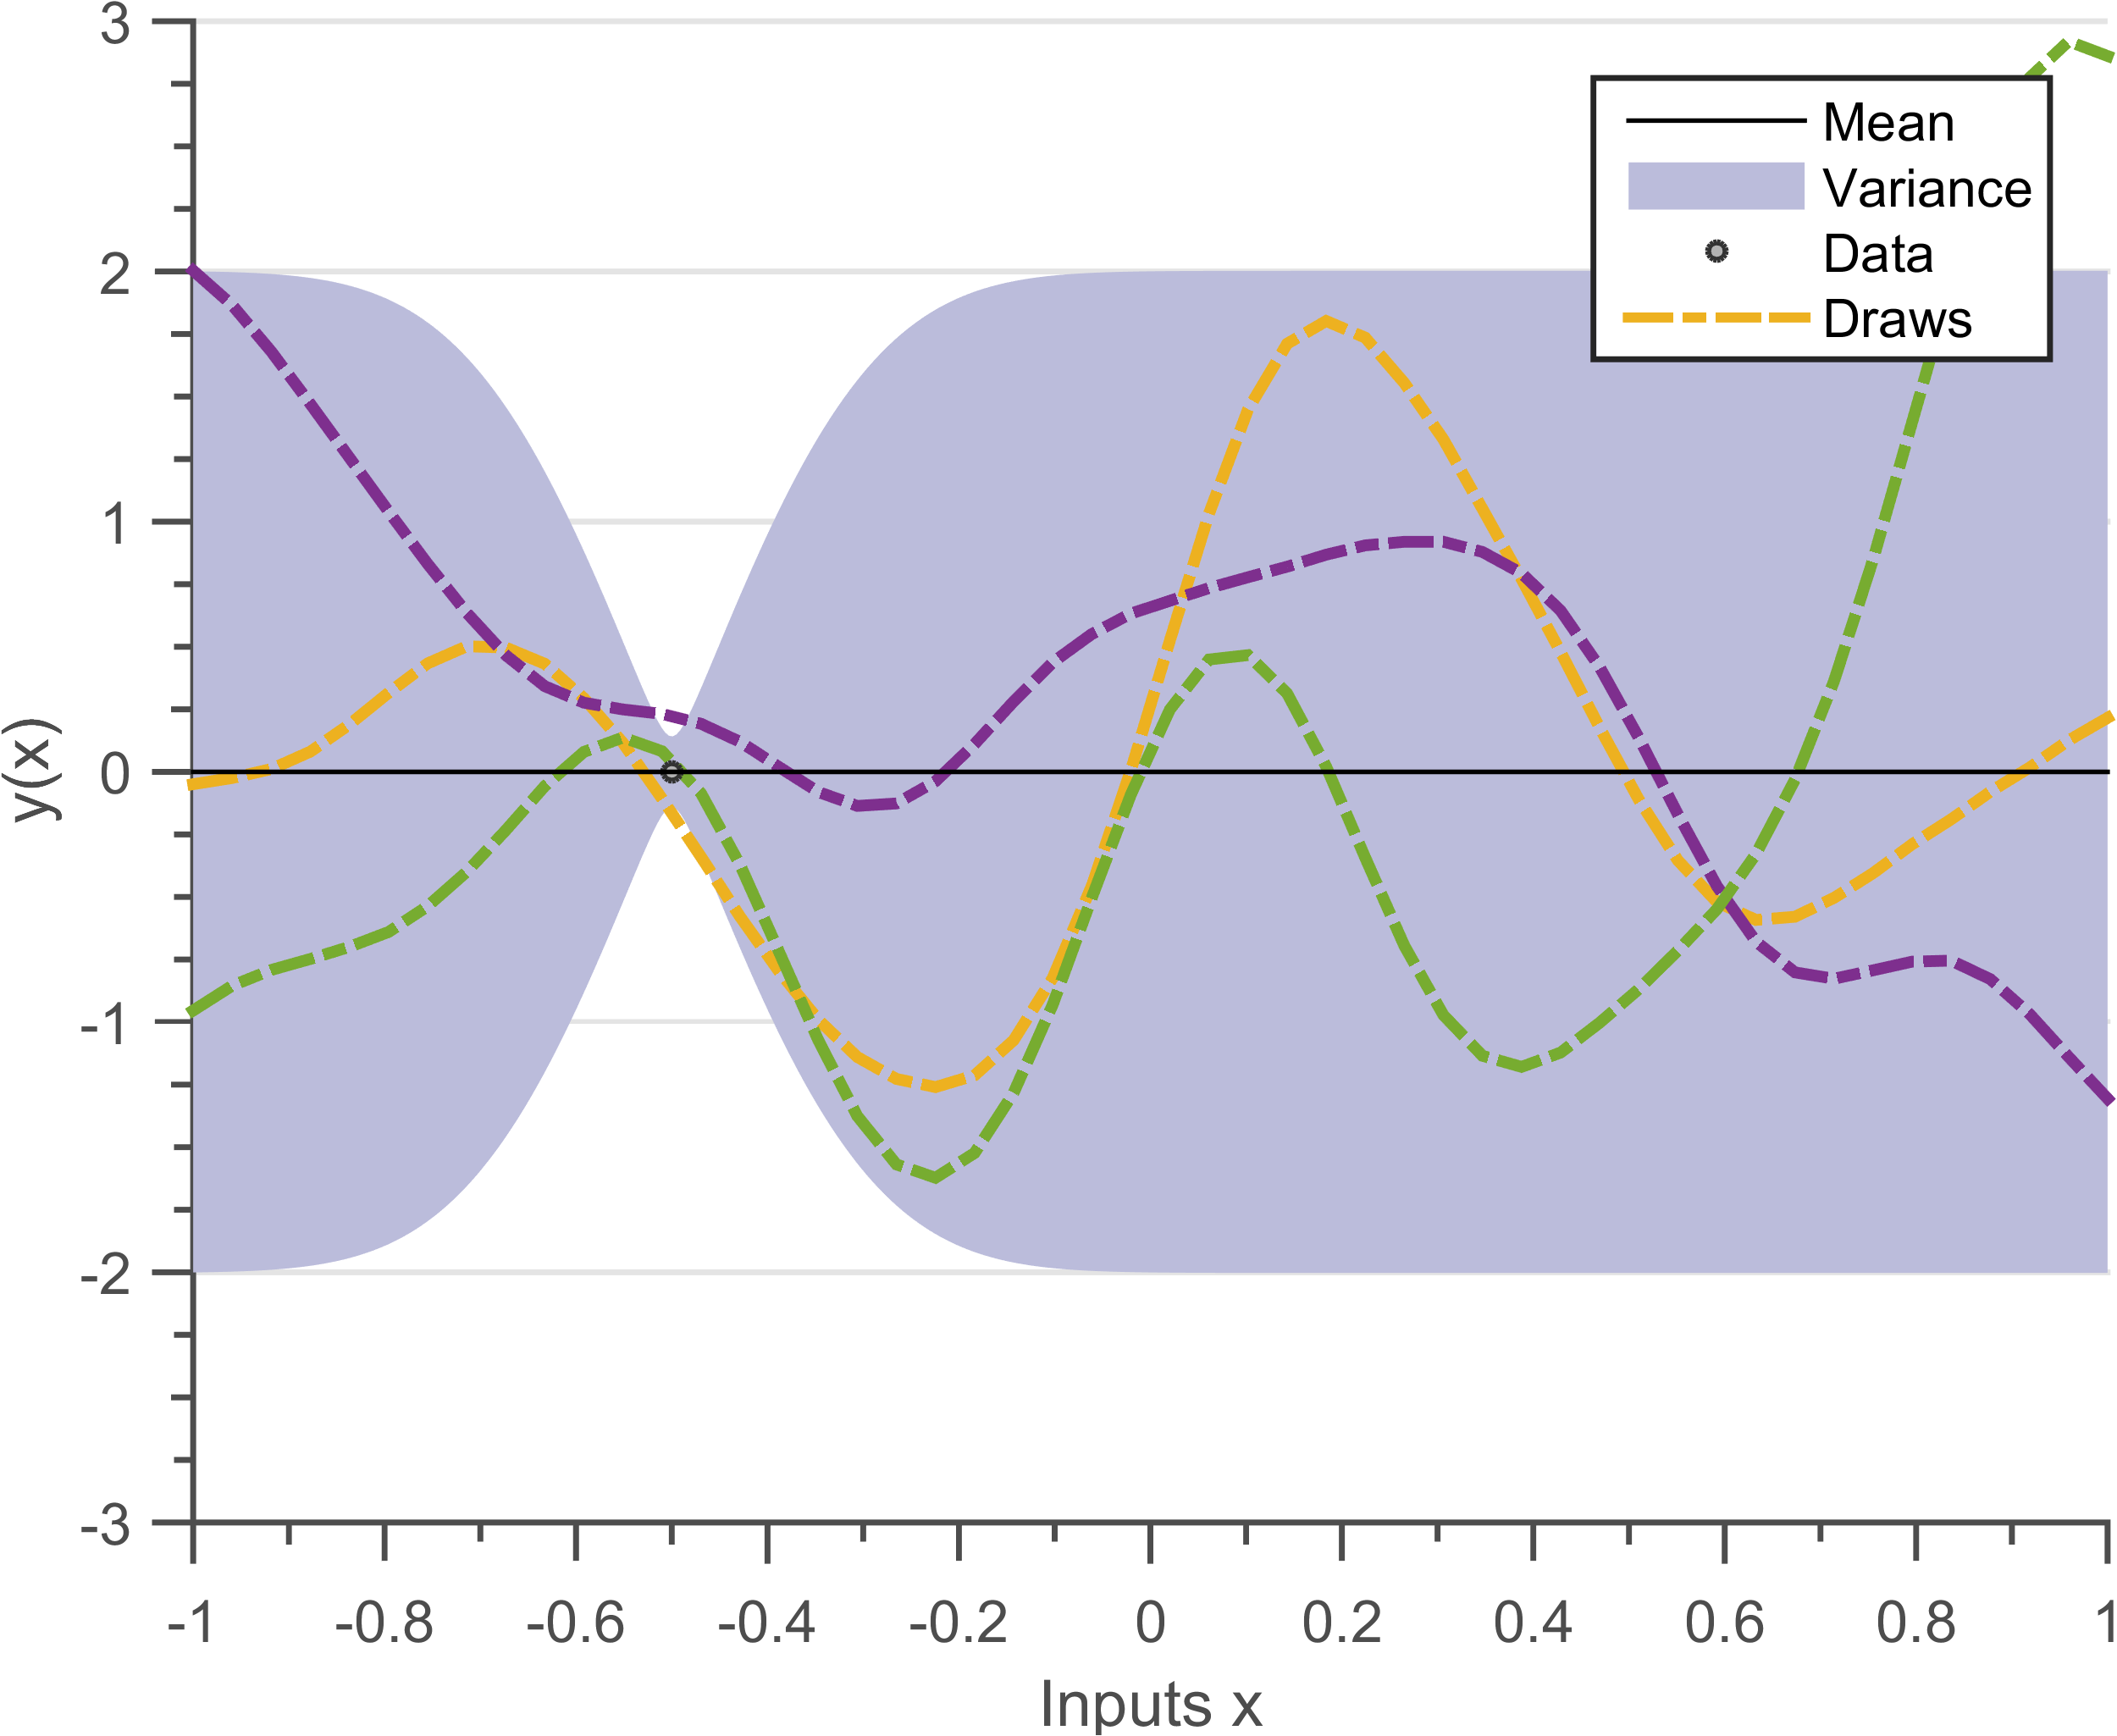
\includegraphics[width=0.45\textwidth]
        {images/part1/posteriorSENoisy_1}
        \label{posteriorSENoisy_1}
  }\quad
\subfigure[{Posterior distribution for the case of noisy observations. Prior is a GP with mean zero, covariance as SE Kernel with $(\VEC{\theta} = [1, 0.2])$ and noise as $\sigma_{n} = [0.02])$, , data set is $\{\VEC{x} = [-0.5, 0.33, 0.66]; \VEC{f} = [0, 0.5, 0.5]\}$.}]
  {
        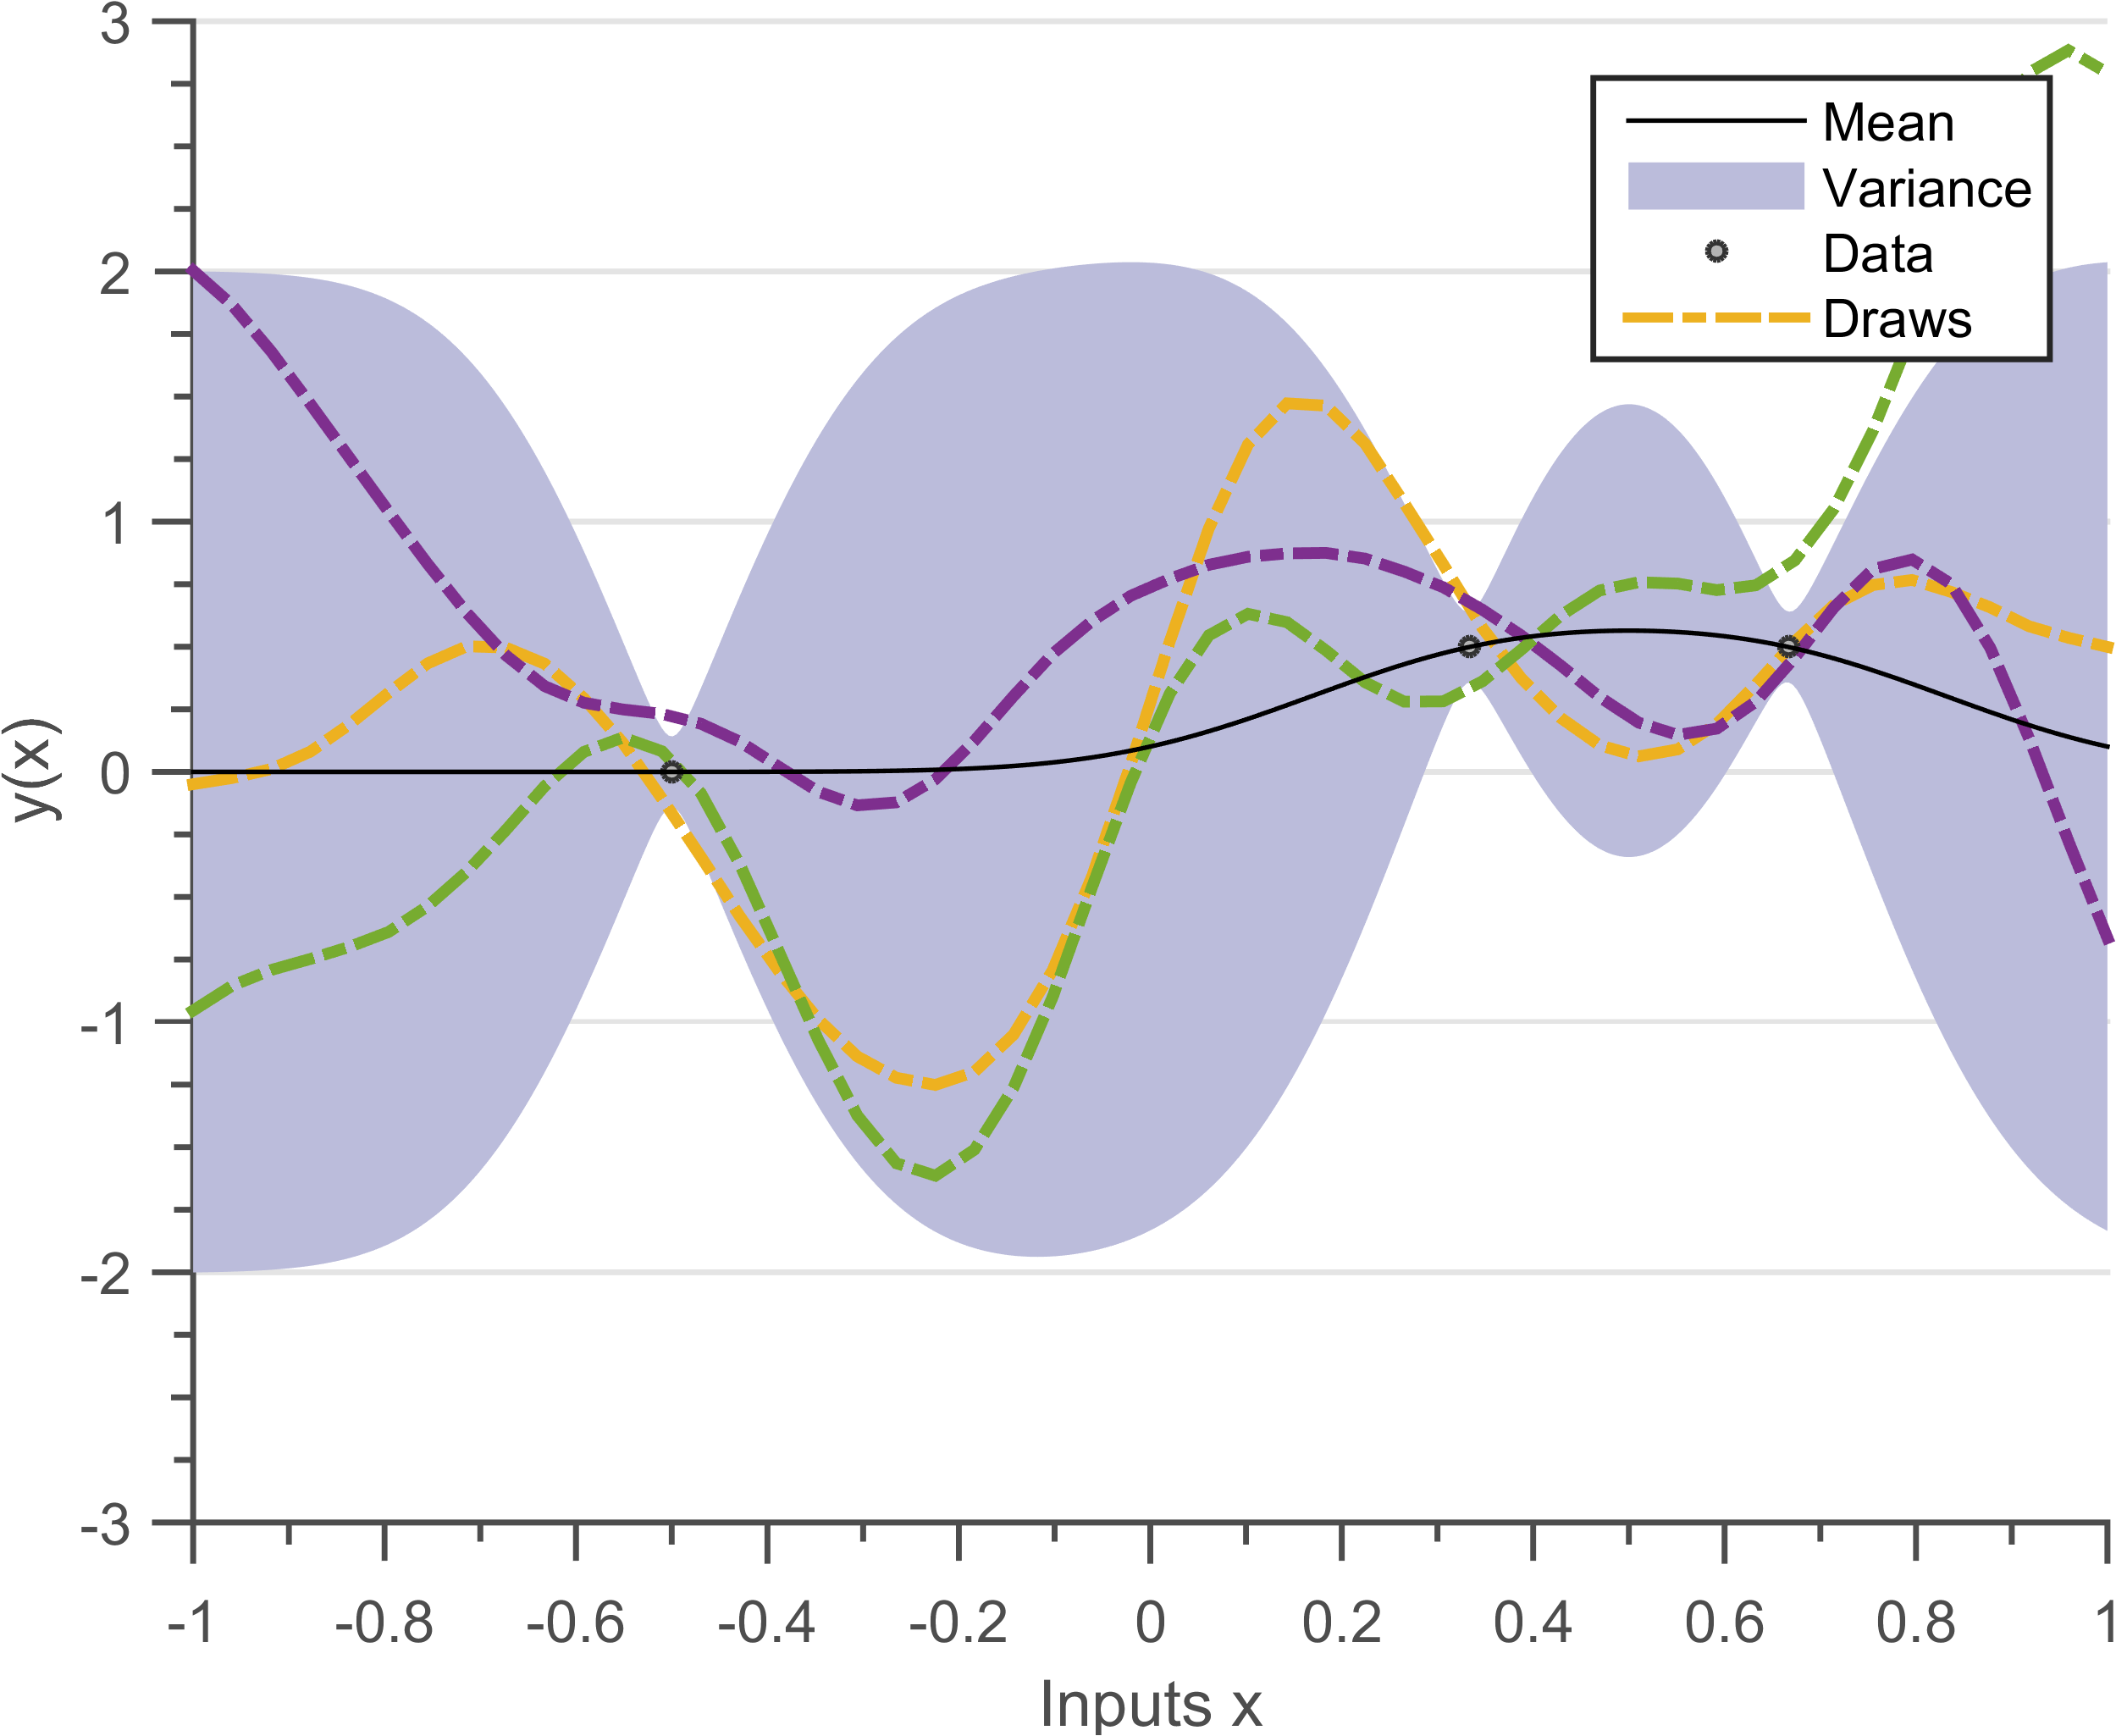
\includegraphics[width=0.45\textwidth]
        {images/part1/posteriorSENoisy_3}
        \label{posteriorSENoisy_3}
  }\quad
  
       \caption{Prediction in the case of noisy observations. The solid black line defines the mean function, blue region defines 95\% confidence interval (2$\sigma$) distance away from the mean. The dashed lines represent three functions drawn at random from a GP posterior. The mean and the draws do not pass exactly from the observation points.}
       \label{figGPNoisyPosteriors}
\end{figure}

\subsection{Interpretation of posterior}
We will now introduce a short hand notation and replace the lengthy notation $\myMatrix{K(X, X)}$ with $\myMatrix{K_{XX}}$ and $\myMatrix{K(X, X_{*})}$ with $\myMatrix{K_{XX_{*}}}$. For the case where we have only one test point $\VEC{x_{*}}$ , we can write the predictive mean and variance in short-hand as:

\begin{equation}\label{eqNoisyPredictiveMean}
  \mathbf{E}[f(\VEC{x_{*}})] = \VEC{k_{Xx_{*}}}^T( \myMatrix{K_{XX}} + \sigma^{2}_{n}\myMatrix{I})^{-1} \VEC{y}
  \end{equation}
  \begin{equation}\label{eqNoisyPredictiveCovariance}
	Cov[f(\VEC{x_{*}})] = k_{x_{*}x_{*}} - \VEC{k_{Xx_{*}}}^{T}( \myMatrix{K_{XX}} + \sigma^{2}_{n}\myMatrix{I} )^{-1} \VEC{k_{Xx_{*}}}
  \end{equation}

\paragraph{Precision Matrix}  
Both the predictive mean (equation \ref{eqNoisyPredictiveMean}) and predictive covariance (equation \ref{eqNoisyPredictiveCovariance}) need the inverse of the covariance matrix $( \myMatrix{K_{XX}} + \sigma^{2}_{n}\myMatrix{I} )^{-1}$. The inverse of a covariance matrix is also known as a precision matrix. While the elements of a covariance matrix capture the variance and correlation information, a precision matrix contains the conditional dependence information \cite{mackay2003information}. Thus, if the $(i, j)^{th}$ element of a precision matrix is zero, the $i^{th}$ and $j^{th}$ random variables are conditionally independent. 

Calculating the precision matrix is an $\mathcal{O}\left ( N^{3} \right )$ operation for a covariance matrix of size $N$. After $N \sim 10,000$ a normal computer runs out of RAM, and thus cannot perform the inversion. Fortunately, there exist several approximations to efficiently invert the covariance matrix and perform predictions, details are available in section \ref{chapScalingGPR}.

\paragraph{Predicted mean}
The predictive mean is a linear combination of the observations $y_{i}$, and factors of $\VEC{k_{Xx_{*}}}^{T}( \myMatrix{K_{XX}} + \sigma^{2}_{n}\myMatrix{I})^{-1}$. Since a SE kernel $\VEC{k_{Xx_{*}}}^{T}$ decreases exponentially with distance, observations closer to $x_{*}$ have more impact on the final prediction (equation \ref{eqNoisyPredictiveMeanLinearInY}). 
  
  \begin{equation}\label{eqNoisyPredictiveMeanLinearInY}
  \mathbf{E}[f(\VEC{x_{*}})] = \sum_{i = 1}^{N} \VEC{k_{Xx_{*}}}^{T}( \myMatrix{K_{XX}} + \sigma^{2}_{n}\myMatrix{I})^{-1} y_{i}
  \end{equation}

The predictive mean can also be interpreted as a linear combination of the basis functions $k_{x_{i}x_{*}} \in \mathbb{R}$, and participation factors $( \myMatrix{K_{XX}} + \sigma^{2}_{n}\myMatrix{I})^{-1}Y$ (equation \ref{eqNoisyPredictiveMeanLinearInBasis}). 

  \begin{equation}\label{eqNoisyPredictiveMeanLinearInBasis}
  \mathbf{E}[f(\VEC{x_{*}})] = \sum_{i = 1}^{N} \VEC{k_{x_{i}x_{*}}}( \myMatrix{K_{XX}} + \sigma^{2}_{n}\myMatrix{I})^{-1} \VEC{y}
  \end{equation}
  
This means that even though a GP represents an infinite-dimensional vector (function), to predict the mean we only care about the $N$ dimensional multivariate Gaussian (section \ref{equationJointPriorNoisy}). If the precision matrix is cached, then calculating the mean is an $\mathcal{O}\left ( N \right )$ operation.

\paragraph{Predicted variance}
The predicted variance is a combination of two terms, $k_{x_{*}x_{*}}$ which is the variance due to prior assumptions, and $- \VEC{k_{Xx_{*}}}^{T}( \myMatrix{K_{XX}} + \sigma^{2}_{n}\myMatrix{I} )^{-1} \VEC{k_{Xx_{*}}}$, which denotes the decrease in variance due to observations. The predictive distribution of test targets $y(x_{*})$ can be calculated by adding a noise term $\sigma^{2}_{n}$ in predictive covariance equation \ref{eqNoisyPredictiveCovariance}. 

  \begin{equation}\label{eqNoisyPredictiveCovarianceOnNoisyTarget}
	Cov[y(\VEC{x_{*}})] = k_{x_{*}x_{*}} - \VEC{k_{Xx_{*}}}^{T}( \myMatrix{K_{XX}} + \sigma^{2}_{n}\myMatrix{I} )^{-1} \VEC{k_{Xx_{*}}} + \sigma_{n}^{2}
  \end{equation}
  
We observe that the predicted variance in not dependent on the observations $y$, this is one of the flaws in GP regression. Since the assumption that the dataset $(\mathcal{D})$ comes from a GP might not necessarily be true, the predicted variance can poorly represent the model error. Hence, predicted variance is not necessarily a measure of model error but an efficient method to track uncertainties arising from the prior assumption and non-continuous observations \cite{shah2014student}.

The mean and variance are highly dependent on the kernel hyper-parameters. In order to automatically learn the hyper-parameters, we must perform model selection. Section \ref{secHyperParameter} details how to fine-tune hyper-parameters to find an optimal prediction.

\section{Choosing Hyper-parameters}\label{secHyperParameter}
Since the properties of functions under a GP are controlled by the functional form of the covariance kernel and its hyper-parameters, model selection amounts to choosing a functional form and learning the hyper-parameters $\VEC{\theta}$ from data. In this section we discuss how to select an optimal model by tuning hyper-parameters for a given covariance function. Please refer to part \ref{partIncorporatePattern} for discussion on how to choose covariance functions. 

We define a new dataset $\mathcal{D}_{2}$ which will be used to compare predictions using different hyper-parameters. The function $f(x)$ (equation \ref{eqFunctionForD2}) is evaluated at 20 equidistant points between $x \in [-1, 1]$ and is corrupted by an independent white noise having variance $\sigma_{noise}^2 = 0.1^2$. Matlab code \ref{codeDatasetD2} is a sample code to generate the dataset  $\mathcal{D}_{2}$. 

\begin{equation}\label{eqFunctionForD2}
f(x) = \frac{sin(5 \pi x)}{5 \pi x}
\end{equation}

\begin{mdframed}[hidealllines=true,backgroundcolor=lightgray!20]
\begin{lstlisting}[caption={Code for dataset D2}, 
                    captionpos=b, 
                    label={codeDatasetD2},
                    style=Matlab-editor,
                    basicstyle=\color{black}\ttfamily\small,
                    backgroundcolor = \color{MatlabCellColour}]
nData = 20; % number of data points

f = @(x)sin(5*pi*x)./(5*pi*x); % Function

noise = 0.1; % Noise in dataset
xData = linspace(-1, 1, nData)';
yData = f(xData) + noise^2*rand(nData, 1);

\end{lstlisting}
\end{mdframed}

Figure \ref{figGPRMarginal} demonstrates that choosing optimal hyper-parameters is very vital for accurate prediction. It compares the posterior distributions obtained for SE priors with two different hyper-parameters. We observe that the mean of figure \ref{subFigPosterior1} passes through all the observed data points but is more complex. The mean in figure \ref{subFigPosterior3} is a smooth function but does not fit the data properly. 

  \begin{figure}[!ht]
  \centering
    \subfigure[{Posterior between SE prior with hyper-parameters $(\VEC{\theta} = [0.35, 0.05]; \sigma_{noise} = 0.01)$ and data. }]
    %$\log (ML) = -35.3$]
  {
        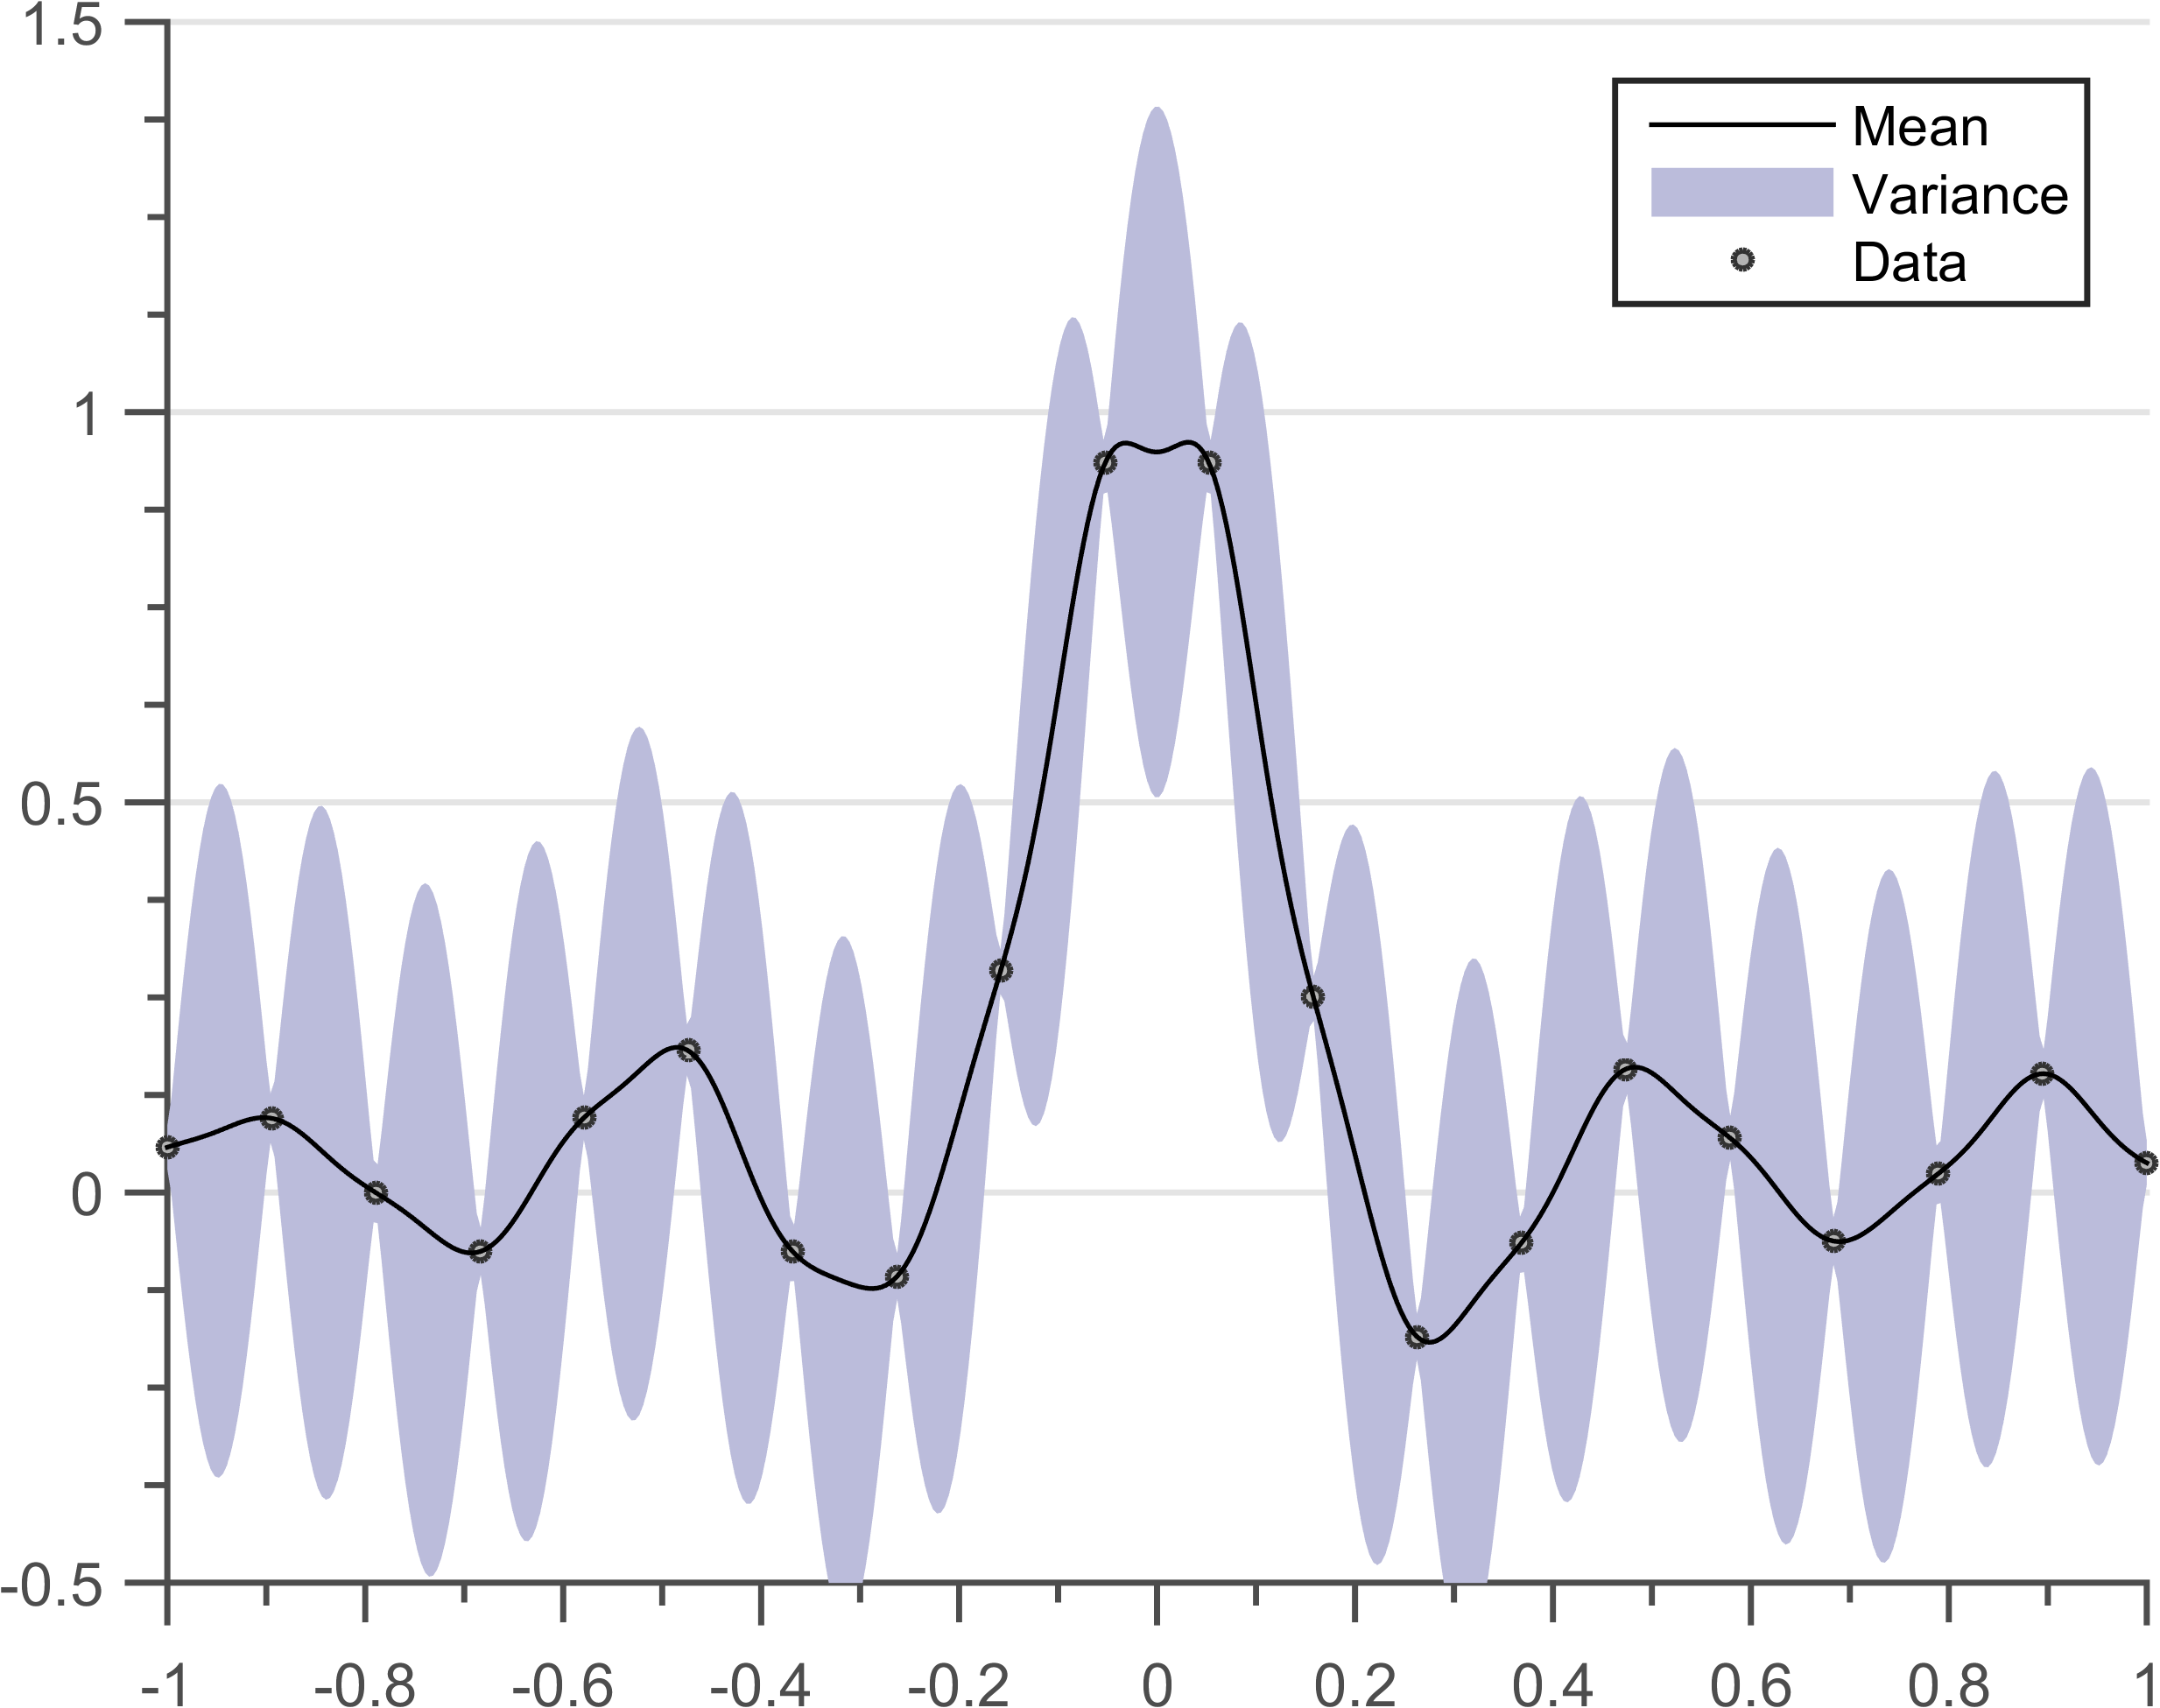
\includegraphics[width=0.45\textwidth]
        {images/part1/posteriorSE1}
        \label{subFigPosterior1}
  }\quad
\subfigure[{Posterior between SE prior with hyper-parameters $(\VEC{\theta} = [0.35, 0.5]; \sigma_{noise} = 0.01)$ and data. }]
%$\log (ML) = -8.2$}]
  {
        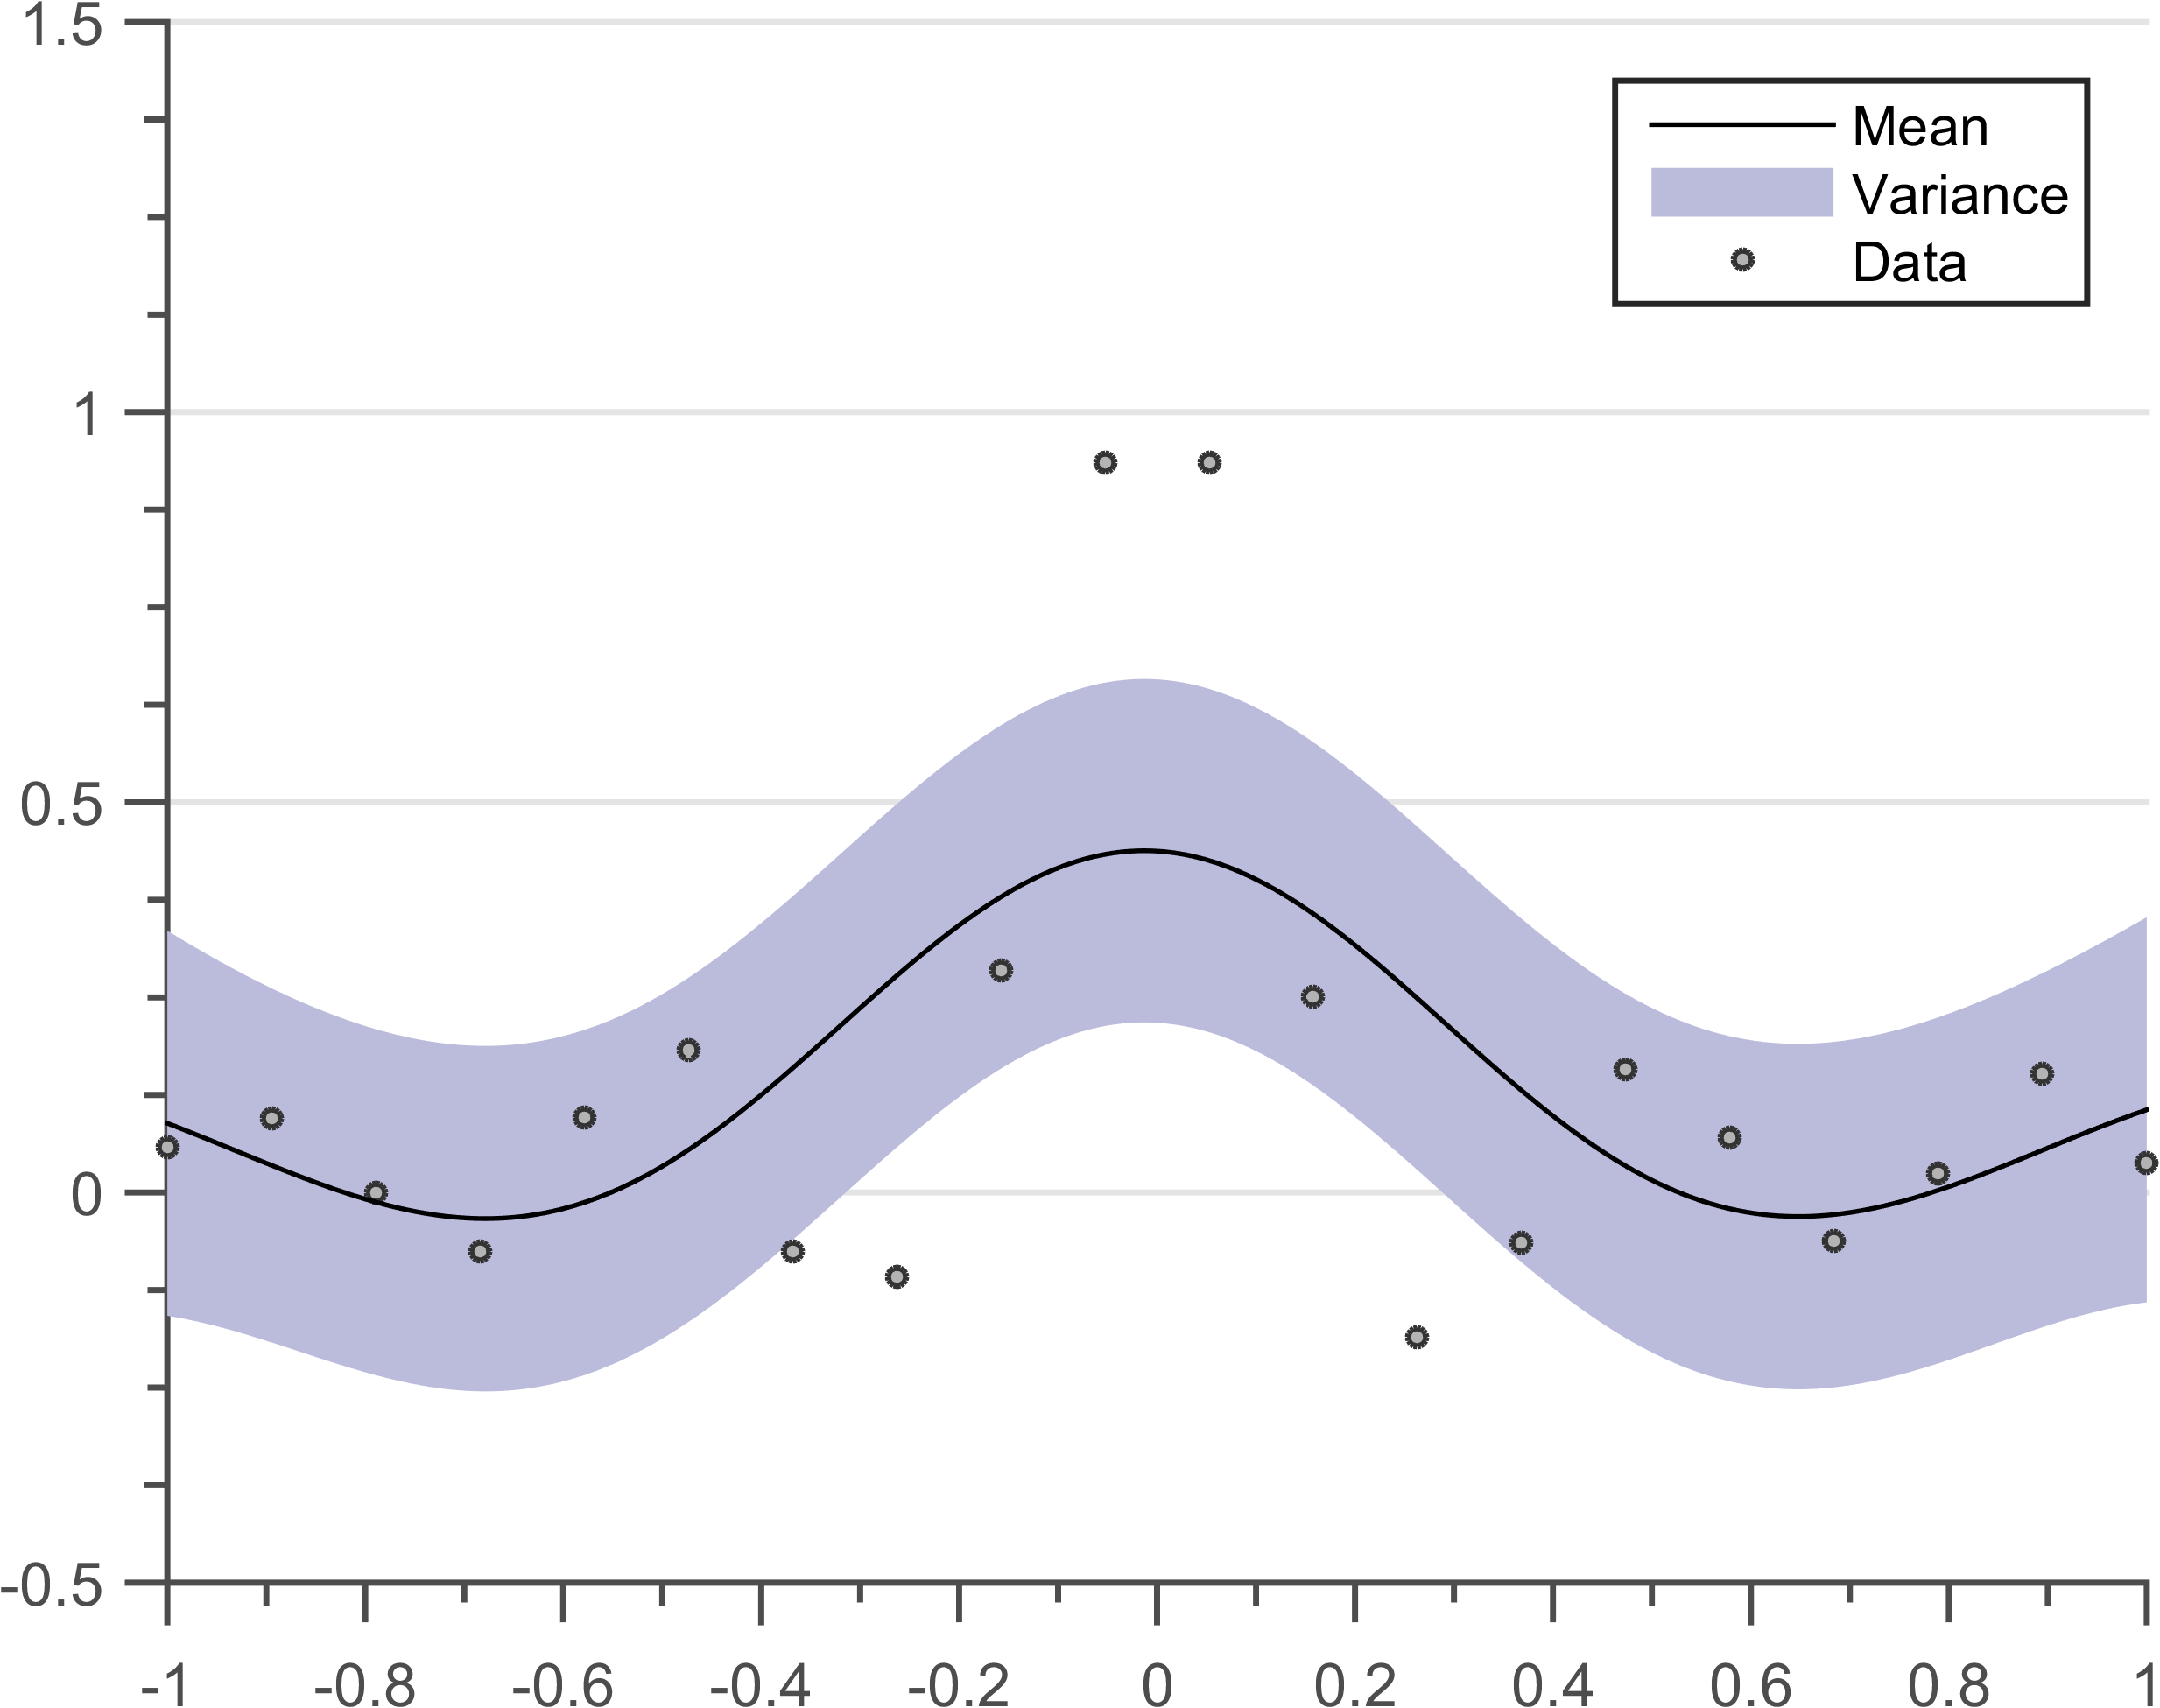
\includegraphics[width=0.45\textwidth]
        {images/part1/posteriorSE3}
        \label{subFigPosterior3}
  }\quad
       \caption{Posteriors for 2 different sets of hyper-parameters. Solid black line defines the mean function, blue region defines 95\% confidence interval (2$\sigma$) distance away from mean. }\label{figGPRMarginal}
\end{figure}

In a pure Bayesian framework we should put a prior over our hyper-parameters $\Pr[\VEC{\theta}]$ and use Bayes Rule to estimate the posterior $\Pr[\VEC{\theta} \mid \myMatrix{X}, \VEC{y}]$ over our data set (just like we did in section \ref{secBayesianModelling}). 

\begin{equation}
    \Pr[\VEC{\theta} \mid \myMatrix{X}, \VEC{y}] = \frac{\Pr[\VEC{y} \mid \myMatrix{X}, \VEC{\theta}] \times \Pr[\VEC{\theta}]}{\Pr[\VEC{y} \mid \myMatrix{X}]}
\end{equation}

The normalizing constant in the denominator (\textit{marginal likelihood}) is given by the following integral.

\begin{equation}
    \Pr[\VEC{y} \mid \myMatrix{X}] = \int \Pr[\VEC{y} \mid \myMatrix{X}, \VEC{\theta}]\Pr[\VEC{\theta}]d\VEC{\theta}
\end{equation}

Depending on the functional form of the covariance function the normalizing constant may or may not be analytically integrable. Hence, approach becomes intractable and several sampling schemes have been proposed to calculate the posterior of hyper-parameters \cite{osborne2010bayesian, neal2011mcmc}.

Another method to find the optimal hyper-parameters is by performing Cross-Validation (CV). CV procedure is to split the experimental design set into two disjoint sets, one is used for training and the other one is used to monitor the performance of the surrogate model. A particular case of CV is the Leave-One-Out (LOO) where test sets are obtained by removing one observation at-a-time \cite{rasmussen2006gaussian, dubrule1983cross, le2013multi}. 

In this manuscript we neither put a prior over our hyper-parameters nor use LOO-CV for choosing hyper-parameters. We use the marginal likelihood, also called evidence, to find optimal hyper-parameters \cite{mackay2003information}. The probability of generating the observations $(\VEC{y})$ at the points $(\myMatrix{X})$ from a prior (defined by $k(\VEC{x_1}, \VEC{x_2}, \VEC{\theta})$) is called the marginal likelihood $\Pr[\VEC{y} \mid \myMatrix{X}, \VEC{\theta}]$. In other words, marginal likelihood is the probability that our data set $\mathcal{D}$ was generated from a particular prior. Hence, when we maximize a marginal likelihood we are finding the best prior that could generate our data set. Using equation \ref{equationMeanZeroGPNoisydefinition} and \ref{equationJointPriorNoisy} we get:

\begin{equation}\label{equationMarginalLikelihood}
\begin{aligned}
\Pr[\VEC{y} \mid \myMatrix{X}, \VEC{\theta}] & = \mathcal{N}(0 , \myMatrix{K(X, X')} + \sigma^{2}_{n}\myMatrix{I})  \\
& = \frac{1}{\sqrt{(2\pi)^{N/2} \myMatrix{K_{XX}}}} exp^{-\frac{1}{2}\VEC{y}^{T}\myMatrix{K_{XX}}\VEC{y}}
\end{aligned}
\end{equation}

Directly maximizing the marginal likelihood with respect to the hyper-parameters can be inefficient. This is because the marginal likelihood does not vary significantly with the hyper-parameters. Hence to speed up the optimization process we generally maximize the log of marginal likelihood \cite{rasmussen2006gaussian}. 

  \begin{equation}\label{eqExactNLML}
\log(\Pr[\VEC{y} \mid \myMatrix{X}, \VEC{\theta}]) = \textcolor{blue}{-\frac{1}{2}\VEC{y}^{T}[\myMatrix{K_{XX}} + \sigma^{2}_{n}\myMatrix{I}]^{-1}\VEC{y}} - \textcolor{red}{\log\left |  \myMatrix{K_{XX}} + \sigma^{2}_{n}\myMatrix{I} \right |} - \textcolor{green}{\frac{N}{2}\log(2\pi)}
  \end{equation}

The log marginal likelihood is composed of three terms a data-fit term $( \textcolor{blue}{-\frac{1}{2}\VEC{y}^{T}[\myMatrix{K_{XX}} + \sigma^{2}_{n}\myMatrix{I}]^{-1}\VEC{y}})$, a model complexity term $( \textcolor{red}{\log\left |  \myMatrix{K_{XX}} + \sigma^{2}_{n}\myMatrix{I} \right |})$, and a normalization term ($\textcolor{green}{\frac{N}{2}\log(2\pi)}$). It performs a trade-off between the data-fit term and the complexity term. The optimization of log marginal likelihood provides the best compromise in terms of explaining the existing data set \{($x_{i}, y_{i}$)\} and the initial assumptions encoded in the prior. The Matlab code \ref{codeOptimizingLML} defines the function `log Marginal Likelihood' (equation \ref{eqExactNLML}), which is maximized later in the code.

\begin{mdframed}[hidealllines=true,backgroundcolor=lightgray!20]
\lstinputlisting[caption={Optimizing the Log Marginal Likelihood}, 
                    captionpos=b, 
                    label={codeOptimizingLML}, 
                    backgroundcolor = \color{MatlabCellColour},
                    style=Matlab-editor,
                    basicstyle=\color{black}\ttfamily\small]
                    {codes/chapter2/optimizingLogMarginalLikelihood.m}
\end{mdframed}

Figure \ref{subFigmaximizingMarginalLikelihood} shows the contours of the marginal likelihood with respect to length-scale $\theta_{lengthScale}$ and noise $\sigma_{n}$ hyper-parameters. The data set is same as used in figure \ref{figGPRMarginal} and the prior is a zero mean with SE kernel. Figure \ref{subFigPosteriorOptimized} shows the posterior for the same data set as used in figure \ref{figGPRMarginal} but for the hyper-parameters where marginal likelihood is maximum. 

  \begin{figure}[!ht]
  \centering
    \subfigure[{Marginal likelihood contours for varying noise and length-scale parameter. The amplitude hyper-parameter is $(\theta_{amplitude} = [0.35])$.  Also shown on the figure are locations of hyper-parameters for figures \ref{subFigPosterior1} and \ref{subFigPosteriorOptimized}.}]
  {
        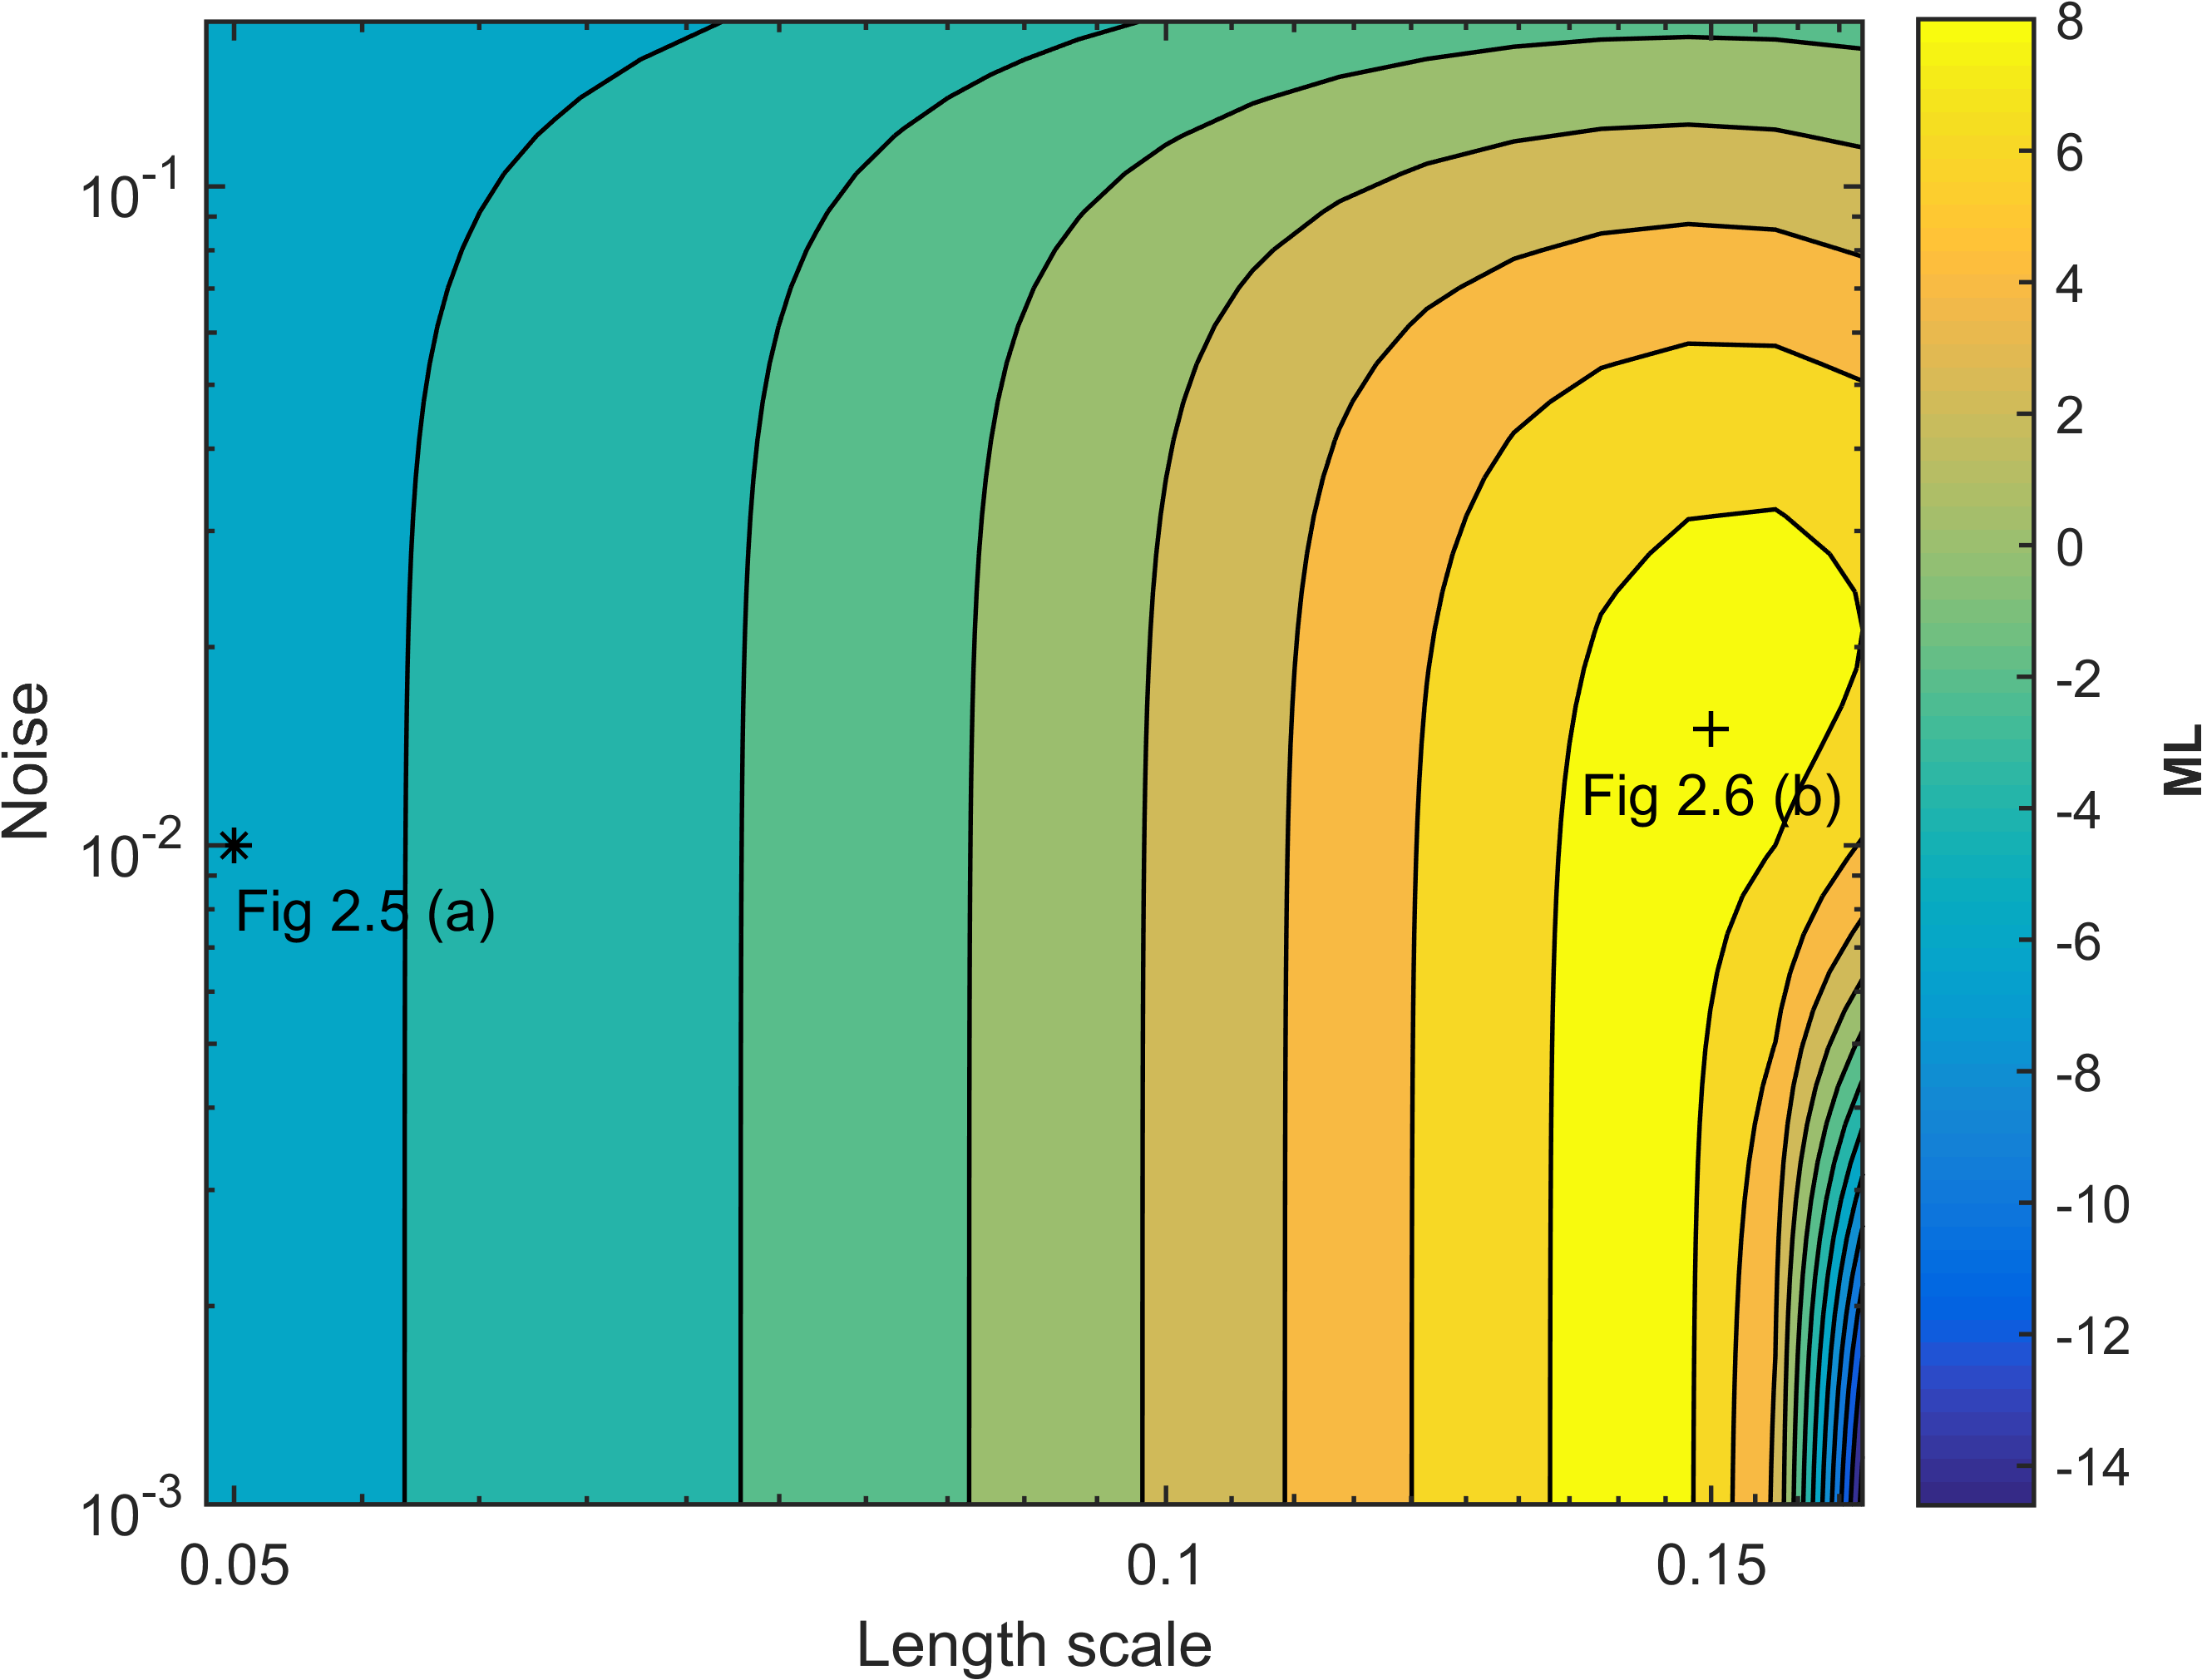
\includegraphics[width=0.45\textwidth]
        {images/part1/maximizingMarginalLikelihood}
        \label{subFigmaximizingMarginalLikelihood}
  }\quad
  \subfigure[{Posterior between SE prior with optimized hyper-parameters $(\theta = [0.35, 0.15]; \sigma_{noise} = 0.015)$ and data. $\log( ML) = 8.04$. Solid black line defines the mean function, blue region defines 95\% confidence interval (2$\sigma$) distance away from mean.}]
  {
        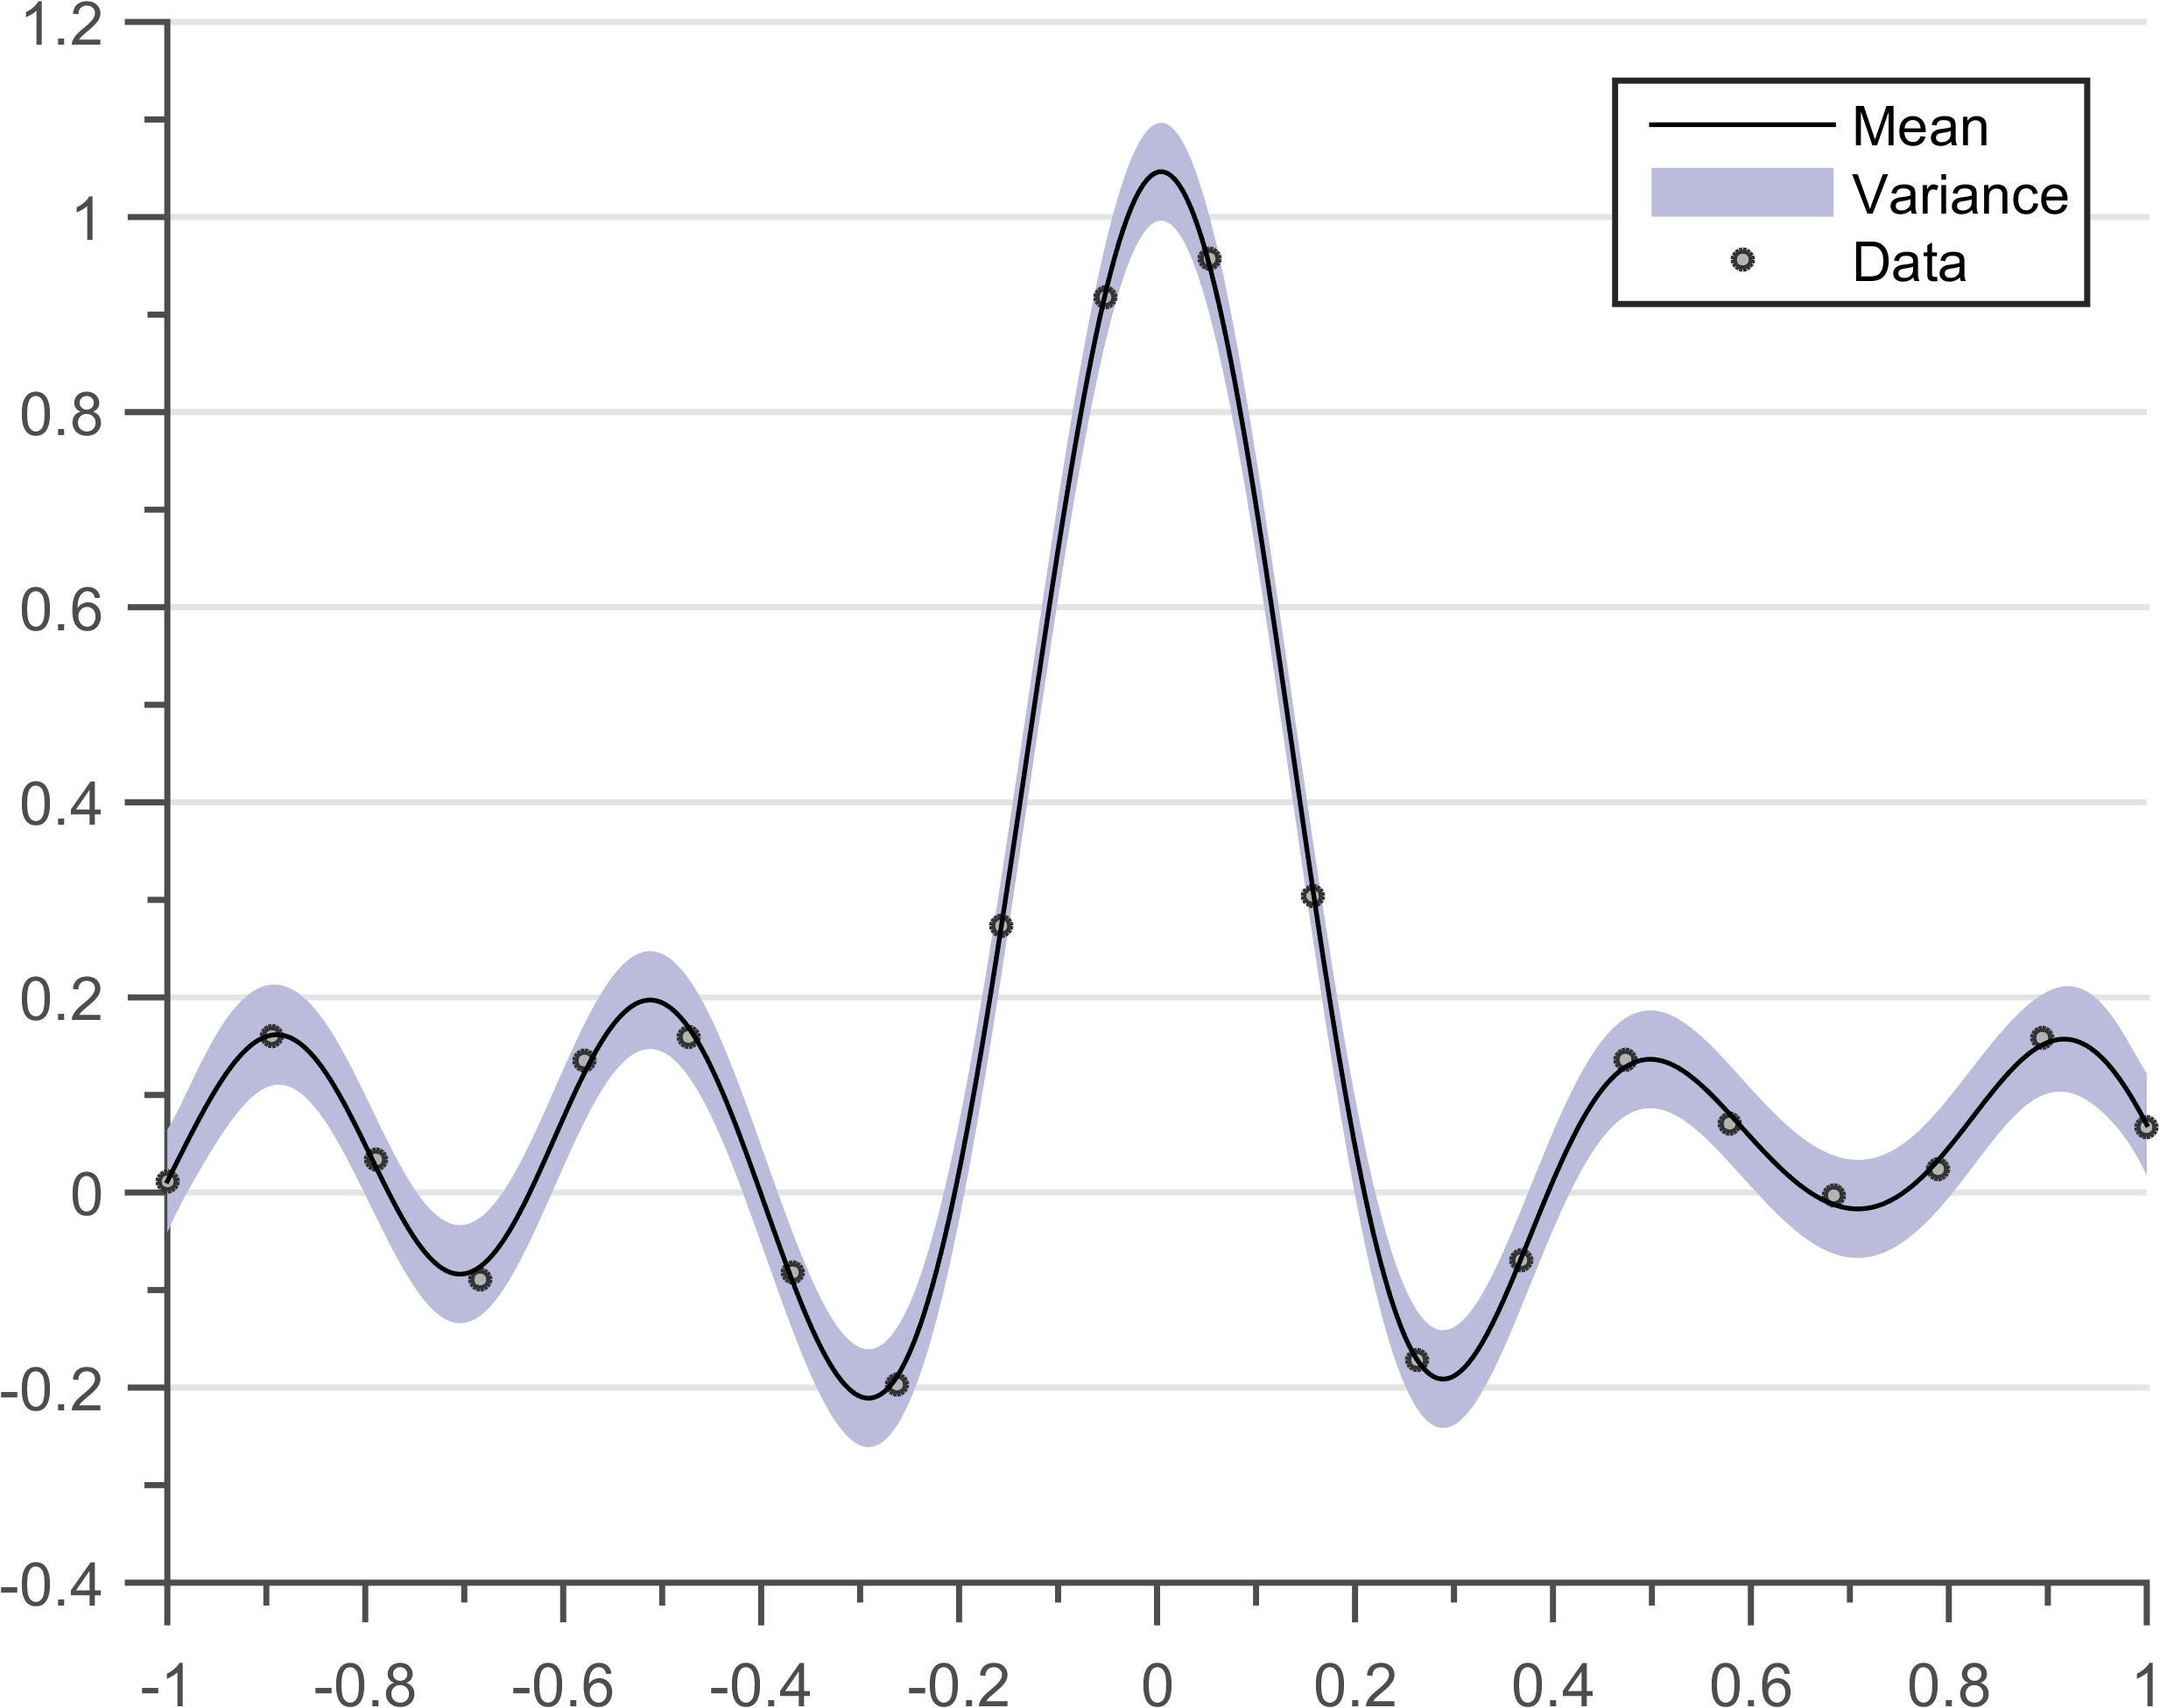
\includegraphics[width=0.45\textwidth]
        {images/part1/posteriorSE}
        \label{subFigPosteriorOptimized}
  }\quad
       \caption{Maximizing marginal likelihood}\label{figGPRMarginalOptimized}
\end{figure}

The marginal likelihood could have multiple maxima in the space of hyper-parameters. Since we do not know \textit{apriori} the multi-modality of log marginal likelihood proper care should be taken while optimizing the hyper-parameters. \cite{forrester2008engineering} propose the use of a global optimizer (genetic algorithm) to find the global optimum, while \cite{le2013multi, bouhlel2016optimisation} propose the use of cross validation to find the global optimum.

\section{Summary and discussion}\label{secCH2Discussion}
In this chapter we provide a brief introduction on how to perform Regression with GPs. GPs are the ideal candidate for regression due to their marginalization property which makes them computationally tractable. Even if GPs define an infinite dimensional random vector, inference on a few points does not require the presence of infinitely other points. This makes drawing functions, calculating posterior distribution, and automating selection of hyper-parameters computationally feasible. This makes GPs an ideal candidate for defining a Prior distribution in a Bayesian Regression framework. 

Section \ref{secPrior} details the key components of the GPs. A GP can be completely parametrized by its mean and covariance function. While the trend of a GP is defined by its mean function, the structure of its constituent functions is defined by the covariance function. The mean of a GP can be assumed to be zero, since an extra term in the covariance function can represent the mean function. Hence the problem of learning in a GP is exactly the problem of finding suitable properties of the covariance function (subsection \ref{subSecCH2Covariance}). Once a function form of covariance is chosen, we can calculate the Gram matrix at desired points and use it to draw random functions from our prior (subsection \ref{subSecSamplingFunctionsGPPrior}). 

Section \ref{secPosterior} describes how to calculate the posterior distribution. The posterior is the conditional distribution $(\Pr[f(\VEC{x_{*}}) \mid \VEC{y}, \myMatrix{X}, \VEC{\theta}])$ for an assumed Prior distribution $(\Pr[f] = GP(0, k(\VEC{x_1}, \VEC{x_2}, \VEC{\theta}))$ and a set of observed data points $(\mathcal{D} = {\myMatrix{X}, \VEC{y}})$. Due to the Gaussian assumption, the conditional probabilities are all computationally tractable and can be calculated using a few matrix operations, side-stepping the computational burden of performing iterative sampling. Calculating the posterior is easy both in the absence (subsection \ref{subSecPosteriorNoiseFree})and presence (subsection \ref{subSecPosteriorNoisy}) of noise in observations. 

Given a functional form of the covariance, section \ref{secHyperParameter} shows the importance of choosing the correct hyper-parameters. In a pure Bayesian framework the posterior distribution of the hyper-parameters should be calculated ($\Pr[\VEC{\theta} \mid \myMatrix{X}, \VEC{y}]$), but this is formally computable, needing several iterations for calculation of integrals. A common practice in the community is maximizing the marginal likelihood to automatically choose the hyper-parameters. Marginal likelihood is the probability of a prior distribution $\Pr[f] = GP(0, k(\VEC{x_1}, \VEC{x_2}, \theta)$ generating the observations $\mathcal{D}$. Hence maximizing the marginal likelihood gives the optimal set of hyper-parameters for a functional form of covariance function (figure \ref{figGPRMarginalOptimized}). 

Calculating the precision matrix $[\myMatrix{K_{XX}}+ \sigma_{noise}^{2}\myMatrix{I}]^{-1}$ is an important task in calculating the marginal likelihood (equation \ref{eqExactNLML}), posterior mean (equation \ref{eqNoisyPredictiveMean}) and covariance (equation \ref{eqNoisyPredictiveCovariance}). Unfortunately, this task has a computational complexity of $\mathcal{O}\left ( N^{3} \right )$ and memory footprint of $\mathcal{O}\left ( N^{2} \right )$. This puts an upper limit of $N \sim 10^4$ on the number of data points, a standard laptop cannot store such a big matrix for inversion \footnote{The computer runs out of memory before we run out of patience :p}. 

In the certification phase of aircraft design, we have access to millions ($N \sim 10^6$) of training data points which depend on several different parameters. \cite{bouhlel2016improved} tackle the problem of building models across several parameters. The next chapter describes few methods of performing approximate inference which scales GPs to $N \sim 10^6$ or more data points. 

